% GNUPLOT: LaTeX picture with Postscript
\begingroup
  \makeatletter
  \providecommand\color[2][]{%
    \GenericError{(gnuplot) \space\space\space\@spaces}{%
      Package color not loaded in conjunction with
      terminal option `colourtext'%
    }{See the gnuplot documentation for explanation.%
    }{Either use 'blacktext' in gnuplot or load the package
      color.sty in LaTeX.}%
    \renewcommand\color[2][]{}%
  }%
  \providecommand\includegraphics[2][]{%
    \GenericError{(gnuplot) \space\space\space\@spaces}{%
      Package graphicx or graphics not loaded%
    }{See the gnuplot documentation for explanation.%
    }{The gnuplot epslatex terminal needs graphicx.sty or graphics.sty.}%
    \renewcommand\includegraphics[2][]{}%
  }%
  \providecommand\rotatebox[2]{#2}%
  \@ifundefined{ifGPcolor}{%
    \newif\ifGPcolor
    \GPcolortrue
  }{}%
  \@ifundefined{ifGPblacktext}{%
    \newif\ifGPblacktext
    \GPblacktexttrue
  }{}%
  % define a \g@addto@macro without @ in the name:
  \let\gplgaddtomacro\g@addto@macro
  % define empty templates for all commands taking text:
  \gdef\gplbacktext{}%
  \gdef\gplfronttext{}%
  \makeatother
  \ifGPblacktext
    % no textcolor at all
    \def\colorrgb#1{}%
    \def\colorgray#1{}%
  \else
    % gray or color?
    \ifGPcolor
      \def\colorrgb#1{\color[rgb]{#1}}%
      \def\colorgray#1{\color[gray]{#1}}%
      \expandafter\def\csname LTw\endcsname{\color{white}}%
      \expandafter\def\csname LTb\endcsname{\color{black}}%
      \expandafter\def\csname LTa\endcsname{\color{black}}%
      \expandafter\def\csname LT0\endcsname{\color[rgb]{1,0,0}}%
      \expandafter\def\csname LT1\endcsname{\color[rgb]{0,1,0}}%
      \expandafter\def\csname LT2\endcsname{\color[rgb]{0,0,1}}%
      \expandafter\def\csname LT3\endcsname{\color[rgb]{1,0,1}}%
      \expandafter\def\csname LT4\endcsname{\color[rgb]{0,1,1}}%
      \expandafter\def\csname LT5\endcsname{\color[rgb]{1,1,0}}%
      \expandafter\def\csname LT6\endcsname{\color[rgb]{0,0,0}}%
      \expandafter\def\csname LT7\endcsname{\color[rgb]{1,0.3,0}}%
      \expandafter\def\csname LT8\endcsname{\color[rgb]{0.5,0.5,0.5}}%
    \else
      % gray
      \def\colorrgb#1{\color{black}}%
      \def\colorgray#1{\color[gray]{#1}}%
      \expandafter\def\csname LTw\endcsname{\color{white}}%
      \expandafter\def\csname LTb\endcsname{\color{black}}%
      \expandafter\def\csname LTa\endcsname{\color{black}}%
      \expandafter\def\csname LT0\endcsname{\color{black}}%
      \expandafter\def\csname LT1\endcsname{\color{black}}%
      \expandafter\def\csname LT2\endcsname{\color{black}}%
      \expandafter\def\csname LT3\endcsname{\color{black}}%
      \expandafter\def\csname LT4\endcsname{\color{black}}%
      \expandafter\def\csname LT5\endcsname{\color{black}}%
      \expandafter\def\csname LT6\endcsname{\color{black}}%
      \expandafter\def\csname LT7\endcsname{\color{black}}%
      \expandafter\def\csname LT8\endcsname{\color{black}}%
    \fi
  \fi
  \setlength{\unitlength}{0.0500bp}%
  \begin{picture}(7200.00,5040.00)%
    \gplgaddtomacro\gplbacktext{%
      \csname LTb\endcsname%
      \put(1342,704){\makebox(0,0)[r]{\strut{} 0}}%
      \put(1342,1317){\makebox(0,0)[r]{\strut{} 0.02}}%
      \put(1342,1929){\makebox(0,0)[r]{\strut{} 0.04}}%
      \put(1342,2542){\makebox(0,0)[r]{\strut{} 0.06}}%
      \put(1342,3155){\makebox(0,0)[r]{\strut{} 0.08}}%
      \put(1342,3767){\makebox(0,0)[r]{\strut{} 0.1}}%
      \put(1342,4380){\makebox(0,0)[r]{\strut{} 0.12}}%
      \put(1474,484){\makebox(0,0){\strut{} 0}}%
      \put(2373,484){\makebox(0,0){\strut{} 0.5}}%
      \put(3273,484){\makebox(0,0){\strut{} 1}}%
      \put(4172,484){\makebox(0,0){\strut{} 1.5}}%
      \put(5071,484){\makebox(0,0){\strut{} 2}}%
      \put(5971,484){\makebox(0,0){\strut{} 2.5}}%
      \put(6870,484){\makebox(0,0){\strut{} 3}}%
      \put(440,2542){\rotatebox{90}{\makebox(0,0){\strut{}I_D}}}%
      \put(4172,154){\makebox(0,0){\strut{}V_GS}}%
      \put(4172,4710){\makebox(0,0){\strut{}I_D=f(V_GS)}}%
    }%
    \gplgaddtomacro\gplfronttext{%
      \csname LTb\endcsname%
      \put(5883,4207){\makebox(0,0)[r]{\strut{}I_D}}%
    }%
    \gplgaddtomacro\gplbacktext{%
      \csname LTb\endcsname%
      \put(1342,704){\makebox(0,0)[r]{\strut{} 0}}%
      \put(1342,1317){\makebox(0,0)[r]{\strut{} 0.02}}%
      \put(1342,1929){\makebox(0,0)[r]{\strut{} 0.04}}%
      \put(1342,2542){\makebox(0,0)[r]{\strut{} 0.06}}%
      \put(1342,3155){\makebox(0,0)[r]{\strut{} 0.08}}%
      \put(1342,3767){\makebox(0,0)[r]{\strut{} 0.1}}%
      \put(1342,4380){\makebox(0,0)[r]{\strut{} 0.12}}%
      \put(1474,484){\makebox(0,0){\strut{} 0}}%
      \put(2373,484){\makebox(0,0){\strut{} 0.5}}%
      \put(3273,484){\makebox(0,0){\strut{} 1}}%
      \put(4172,484){\makebox(0,0){\strut{} 1.5}}%
      \put(5071,484){\makebox(0,0){\strut{} 2}}%
      \put(5971,484){\makebox(0,0){\strut{} 2.5}}%
      \put(6870,484){\makebox(0,0){\strut{} 3}}%
      \put(440,2542){\rotatebox{90}{\makebox(0,0){\strut{}I_D}}}%
      \put(4172,154){\makebox(0,0){\strut{}V_GS}}%
      \put(4172,4710){\makebox(0,0){\strut{}I_D=f(V_GS)}}%
    }%
    \gplgaddtomacro\gplfronttext{%
      \csname LTb\endcsname%
      \put(5883,4207){\makebox(0,0)[r]{\strut{}I_D}}%
    }%
    \gplgaddtomacro\gplbacktext{%
      \csname LTb\endcsname%
      \put(1342,704){\makebox(0,0)[r]{\strut{} 0}}%
      \put(1342,1317){\makebox(0,0)[r]{\strut{} 0.02}}%
      \put(1342,1929){\makebox(0,0)[r]{\strut{} 0.04}}%
      \put(1342,2542){\makebox(0,0)[r]{\strut{} 0.06}}%
      \put(1342,3155){\makebox(0,0)[r]{\strut{} 0.08}}%
      \put(1342,3767){\makebox(0,0)[r]{\strut{} 0.1}}%
      \put(1342,4380){\makebox(0,0)[r]{\strut{} 0.12}}%
      \put(1474,484){\makebox(0,0){\strut{} 0}}%
      \put(2373,484){\makebox(0,0){\strut{} 0.5}}%
      \put(3273,484){\makebox(0,0){\strut{} 1}}%
      \put(4172,484){\makebox(0,0){\strut{} 1.5}}%
      \put(5071,484){\makebox(0,0){\strut{} 2}}%
      \put(5971,484){\makebox(0,0){\strut{} 2.5}}%
      \put(6870,484){\makebox(0,0){\strut{} 3}}%
      \put(440,2542){\rotatebox{90}{\makebox(0,0){\strut{}I_D}}}%
      \put(4172,154){\makebox(0,0){\strut{}V_{GS}}}%
      \put(4172,4710){\makebox(0,0){\strut{}I_D=f(V_{GS})}}%
    }%
    \gplgaddtomacro\gplfronttext{%
      \csname LTb\endcsname%
      \put(5883,4207){\makebox(0,0)[r]{\strut{}I_D}}%
    }%
    \gplgaddtomacro\gplbacktext{%
      \csname LTb\endcsname%
      \put(1342,704){\makebox(0,0)[r]{\strut{} 0}}%
      \csname LTb\endcsname%
      \put(1342,1317){\makebox(0,0)[r]{\strut{} 0.02}}%
      \csname LTb\endcsname%
      \put(1342,1929){\makebox(0,0)[r]{\strut{} 0.04}}%
      \csname LTb\endcsname%
      \put(1342,2542){\makebox(0,0)[r]{\strut{} 0.06}}%
      \csname LTb\endcsname%
      \put(1342,3155){\makebox(0,0)[r]{\strut{} 0.08}}%
      \csname LTb\endcsname%
      \put(1342,3767){\makebox(0,0)[r]{\strut{} 0.1}}%
      \csname LTb\endcsname%
      \put(1342,4380){\makebox(0,0)[r]{\strut{} 0.12}}%
      \csname LTb\endcsname%
      \put(1474,484){\makebox(0,0){\strut{} 0}}%
      \csname LTb\endcsname%
      \put(2373,484){\makebox(0,0){\strut{} 0.5}}%
      \csname LTb\endcsname%
      \put(3273,484){\makebox(0,0){\strut{} 1}}%
      \csname LTb\endcsname%
      \put(4172,484){\makebox(0,0){\strut{} 1.5}}%
      \csname LTb\endcsname%
      \put(5071,484){\makebox(0,0){\strut{} 2}}%
      \csname LTb\endcsname%
      \put(5971,484){\makebox(0,0){\strut{} 2.5}}%
      \csname LTb\endcsname%
      \put(6870,484){\makebox(0,0){\strut{} 3}}%
      \put(440,2542){\rotatebox{90}{\makebox(0,0){\strut{}I_D}}}%
      \put(4172,154){\makebox(0,0){\strut{}V_{GS}}}%
      \put(4172,4710){\makebox(0,0){\strut{}I_D=f(V_{GS})}}%
    }%
    \gplgaddtomacro\gplfronttext{%
      \csname LTb\endcsname%
      \put(5883,4207){\makebox(0,0)[r]{\strut{}I_D}}%
    }%
    \gplgaddtomacro\gplbacktext{%
      \csname LTb\endcsname%
      \put(1342,704){\makebox(0,0)[r]{\strut{} 0}}%
      \csname LTb\endcsname%
      \put(1342,1317){\makebox(0,0)[r]{\strut{} 0.02}}%
      \csname LTb\endcsname%
      \put(1342,1929){\makebox(0,0)[r]{\strut{} 0.04}}%
      \csname LTb\endcsname%
      \put(1342,2542){\makebox(0,0)[r]{\strut{} 0.06}}%
      \csname LTb\endcsname%
      \put(1342,3155){\makebox(0,0)[r]{\strut{} 0.08}}%
      \csname LTb\endcsname%
      \put(1342,3767){\makebox(0,0)[r]{\strut{} 0.1}}%
      \csname LTb\endcsname%
      \put(1342,4380){\makebox(0,0)[r]{\strut{} 0.12}}%
      \csname LTb\endcsname%
      \put(1474,484){\makebox(0,0){\strut{} 0}}%
      \csname LTb\endcsname%
      \put(2373,484){\makebox(0,0){\strut{} 0.5}}%
      \csname LTb\endcsname%
      \put(3273,484){\makebox(0,0){\strut{} 1}}%
      \csname LTb\endcsname%
      \put(4172,484){\makebox(0,0){\strut{} 1.5}}%
      \csname LTb\endcsname%
      \put(5071,484){\makebox(0,0){\strut{} 2}}%
      \csname LTb\endcsname%
      \put(5971,484){\makebox(0,0){\strut{} 2.5}}%
      \csname LTb\endcsname%
      \put(6870,484){\makebox(0,0){\strut{} 3}}%
      \put(440,2542){\rotatebox{90}{\makebox(0,0){\strut{}I_D}}}%
      \put(4172,154){\makebox(0,0){\strut{}V_{GS}}}%
      \put(4172,4710){\makebox(0,0){\strut{}I_D=f(V_{GS})}}%
    }%
    \gplgaddtomacro\gplfronttext{%
      \csname LTb\endcsname%
      \put(5883,4207){\makebox(0,0)[r]{\strut{}I_D}}%
    }%
    \gplbacktext
    \put(0,0){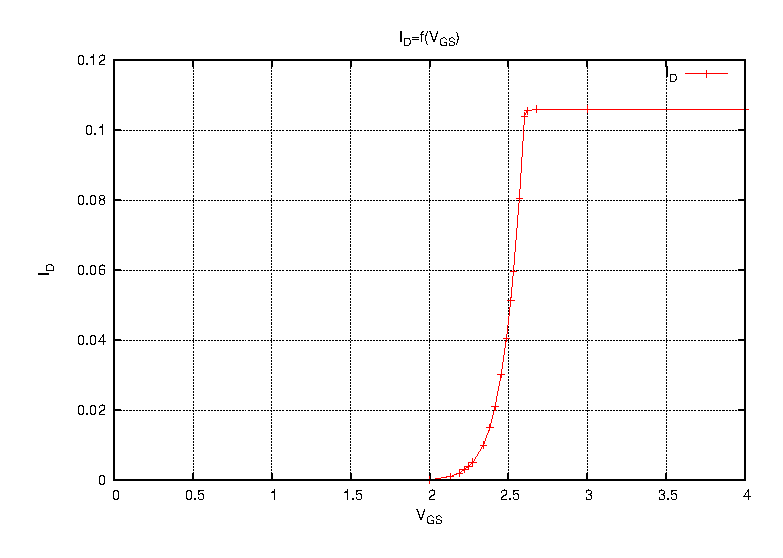
\includegraphics{id_vgs}}%
    \gplfronttext
  \end{picture}%
\endgroup
%!PS-Adobe-2.0
%%Title: id_vgs.tex
%%Creator: gnuplot 4.2 patchlevel 6 
%%CreationDate: Wed Dec 15 00:23:07 2010
%%DocumentFonts: (atend)
%%BoundingBox: 50 50 554 770
%%Orientation: Landscape
%%Pages: (atend)
%%EndComments
%%BeginProlog
/gnudict 256 dict def
gnudict begin
%
% The following 6 true/false flags may be edited by hand if required
% The unit line width may also be changed
%
/Color true def
/Blacktext false def
/Solid false def
/Dashlength 1 def
/Landscape true def
/Level1 false def
/Rounded false def
/TransparentPatterns false def
/gnulinewidth 5.000 def
/userlinewidth gnulinewidth def
%
/vshift -46 def
/dl1 {
  10.0 Dashlength mul mul
  Rounded { currentlinewidth 0.75 mul sub dup 0 le { pop 0.01 } if } if
} def
/dl2 {
  10.0 Dashlength mul mul
  Rounded { currentlinewidth 0.75 mul add } if
} def
/hpt_ 31.5 def
/vpt_ 31.5 def
/hpt hpt_ def
/vpt vpt_ def
Level1 {} {
/SDict 10 dict def
systemdict /pdfmark known not {
  userdict /pdfmark systemdict /cleartomark get put
} if
SDict begin [
  /Title (id_vgs.tex)
  /Subject (gnuplot plot)
  /Creator (gnuplot 4.2 patchlevel 6 )
  /Author (yallard)
%  /Producer (gnuplot)
%  /Keywords ()
  /CreationDate (Wed Dec 15 00:23:07 2010)
  /DOCINFO pdfmark
end
} ifelse
%
% Gnuplot Prolog Version 4.2 (August 2006)
%
/M {moveto} bind def
/L {lineto} bind def
/R {rmoveto} bind def
/V {rlineto} bind def
/N {newpath moveto} bind def
/Z {closepath} bind def
/C {setrgbcolor} bind def
/f {rlineto fill} bind def
/vpt2 vpt 2 mul def
/hpt2 hpt 2 mul def
/Lshow {currentpoint stroke M 0 vshift R 
	Blacktext {gsave 0 setgray show grestore} {show} ifelse} def
/Rshow {currentpoint stroke M dup stringwidth pop neg vshift R
	Blacktext {gsave 0 setgray show grestore} {show} ifelse} def
/Cshow {currentpoint stroke M dup stringwidth pop -2 div vshift R 
	Blacktext {gsave 0 setgray show grestore} {show} ifelse} def
/UP {dup vpt_ mul /vpt exch def hpt_ mul /hpt exch def
  /hpt2 hpt 2 mul def /vpt2 vpt 2 mul def} def
/DL {Color {setrgbcolor Solid {pop []} if 0 setdash}
 {pop pop pop 0 setgray Solid {pop []} if 0 setdash} ifelse} def
/BL {stroke userlinewidth 2 mul setlinewidth
	Rounded {1 setlinejoin 1 setlinecap} if} def
/AL {stroke userlinewidth 2 div setlinewidth
	Rounded {1 setlinejoin 1 setlinecap} if} def
/UL {dup gnulinewidth mul /userlinewidth exch def
	dup 1 lt {pop 1} if 10 mul /udl exch def} def
/PL {stroke userlinewidth setlinewidth
	Rounded {1 setlinejoin 1 setlinecap} if} def
% Default Line colors
/LCw {1 1 1} def
/LCb {0 0 0} def
/LCa {0 0 0} def
/LC0 {1 0 0} def
/LC1 {0 1 0} def
/LC2 {0 0 1} def
/LC3 {1 0 1} def
/LC4 {0 1 1} def
/LC5 {1 1 0} def
/LC6 {0 0 0} def
/LC7 {1 0.3 0} def
/LC8 {0.5 0.5 0.5} def
% Default Line Types
/LTw {PL [] 1 setgray} def
/LTb {BL [] LCb DL} def
/LTa {AL [1 udl mul 2 udl mul] 0 setdash LCa setrgbcolor} def
/LT0 {PL [] LC0 DL} def
/LT1 {PL [4 dl1 2 dl2] LC1 DL} def
/LT2 {PL [2 dl1 3 dl2] LC2 DL} def
/LT3 {PL [1 dl1 1.5 dl2] LC3 DL} def
/LT4 {PL [6 dl1 2 dl2 1 dl1 2 dl2] LC4 DL} def
/LT5 {PL [3 dl1 3 dl2 1 dl1 3 dl2] LC5 DL} def
/LT6 {PL [2 dl1 2 dl2 2 dl1 6 dl2] LC6 DL} def
/LT7 {PL [1 dl1 2 dl2 6 dl1 2 dl2 1 dl1 2 dl2] LC7 DL} def
/LT8 {PL [2 dl1 2 dl2 2 dl1 2 dl2 2 dl1 2 dl2 2 dl1 4 dl2] LC8 DL} def
/Pnt {stroke [] 0 setdash gsave 1 setlinecap M 0 0 V stroke grestore} def
/Dia {stroke [] 0 setdash 2 copy vpt add M
  hpt neg vpt neg V hpt vpt neg V
  hpt vpt V hpt neg vpt V closepath stroke
  Pnt} def
/Pls {stroke [] 0 setdash vpt sub M 0 vpt2 V
  currentpoint stroke M
  hpt neg vpt neg R hpt2 0 V stroke
 } def
/Box {stroke [] 0 setdash 2 copy exch hpt sub exch vpt add M
  0 vpt2 neg V hpt2 0 V 0 vpt2 V
  hpt2 neg 0 V closepath stroke
  Pnt} def
/Crs {stroke [] 0 setdash exch hpt sub exch vpt add M
  hpt2 vpt2 neg V currentpoint stroke M
  hpt2 neg 0 R hpt2 vpt2 V stroke} def
/TriU {stroke [] 0 setdash 2 copy vpt 1.12 mul add M
  hpt neg vpt -1.62 mul V
  hpt 2 mul 0 V
  hpt neg vpt 1.62 mul V closepath stroke
  Pnt} def
/Star {2 copy Pls Crs} def
/BoxF {stroke [] 0 setdash exch hpt sub exch vpt add M
  0 vpt2 neg V hpt2 0 V 0 vpt2 V
  hpt2 neg 0 V closepath fill} def
/TriUF {stroke [] 0 setdash vpt 1.12 mul add M
  hpt neg vpt -1.62 mul V
  hpt 2 mul 0 V
  hpt neg vpt 1.62 mul V closepath fill} def
/TriD {stroke [] 0 setdash 2 copy vpt 1.12 mul sub M
  hpt neg vpt 1.62 mul V
  hpt 2 mul 0 V
  hpt neg vpt -1.62 mul V closepath stroke
  Pnt} def
/TriDF {stroke [] 0 setdash vpt 1.12 mul sub M
  hpt neg vpt 1.62 mul V
  hpt 2 mul 0 V
  hpt neg vpt -1.62 mul V closepath fill} def
/DiaF {stroke [] 0 setdash vpt add M
  hpt neg vpt neg V hpt vpt neg V
  hpt vpt V hpt neg vpt V closepath fill} def
/Pent {stroke [] 0 setdash 2 copy gsave
  translate 0 hpt M 4 {72 rotate 0 hpt L} repeat
  closepath stroke grestore Pnt} def
/PentF {stroke [] 0 setdash gsave
  translate 0 hpt M 4 {72 rotate 0 hpt L} repeat
  closepath fill grestore} def
/Circle {stroke [] 0 setdash 2 copy
  hpt 0 360 arc stroke Pnt} def
/CircleF {stroke [] 0 setdash hpt 0 360 arc fill} def
/C0 {BL [] 0 setdash 2 copy moveto vpt 90 450 arc} bind def
/C1 {BL [] 0 setdash 2 copy moveto
	2 copy vpt 0 90 arc closepath fill
	vpt 0 360 arc closepath} bind def
/C2 {BL [] 0 setdash 2 copy moveto
	2 copy vpt 90 180 arc closepath fill
	vpt 0 360 arc closepath} bind def
/C3 {BL [] 0 setdash 2 copy moveto
	2 copy vpt 0 180 arc closepath fill
	vpt 0 360 arc closepath} bind def
/C4 {BL [] 0 setdash 2 copy moveto
	2 copy vpt 180 270 arc closepath fill
	vpt 0 360 arc closepath} bind def
/C5 {BL [] 0 setdash 2 copy moveto
	2 copy vpt 0 90 arc
	2 copy moveto
	2 copy vpt 180 270 arc closepath fill
	vpt 0 360 arc} bind def
/C6 {BL [] 0 setdash 2 copy moveto
	2 copy vpt 90 270 arc closepath fill
	vpt 0 360 arc closepath} bind def
/C7 {BL [] 0 setdash 2 copy moveto
	2 copy vpt 0 270 arc closepath fill
	vpt 0 360 arc closepath} bind def
/C8 {BL [] 0 setdash 2 copy moveto
	2 copy vpt 270 360 arc closepath fill
	vpt 0 360 arc closepath} bind def
/C9 {BL [] 0 setdash 2 copy moveto
	2 copy vpt 270 450 arc closepath fill
	vpt 0 360 arc closepath} bind def
/C10 {BL [] 0 setdash 2 copy 2 copy moveto vpt 270 360 arc closepath fill
	2 copy moveto
	2 copy vpt 90 180 arc closepath fill
	vpt 0 360 arc closepath} bind def
/C11 {BL [] 0 setdash 2 copy moveto
	2 copy vpt 0 180 arc closepath fill
	2 copy moveto
	2 copy vpt 270 360 arc closepath fill
	vpt 0 360 arc closepath} bind def
/C12 {BL [] 0 setdash 2 copy moveto
	2 copy vpt 180 360 arc closepath fill
	vpt 0 360 arc closepath} bind def
/C13 {BL [] 0 setdash 2 copy moveto
	2 copy vpt 0 90 arc closepath fill
	2 copy moveto
	2 copy vpt 180 360 arc closepath fill
	vpt 0 360 arc closepath} bind def
/C14 {BL [] 0 setdash 2 copy moveto
	2 copy vpt 90 360 arc closepath fill
	vpt 0 360 arc} bind def
/C15 {BL [] 0 setdash 2 copy vpt 0 360 arc closepath fill
	vpt 0 360 arc closepath} bind def
/Rec {newpath 4 2 roll moveto 1 index 0 rlineto 0 exch rlineto
	neg 0 rlineto closepath} bind def
/Square {dup Rec} bind def
/Bsquare {vpt sub exch vpt sub exch vpt2 Square} bind def
/S0 {BL [] 0 setdash 2 copy moveto 0 vpt rlineto BL Bsquare} bind def
/S1 {BL [] 0 setdash 2 copy vpt Square fill Bsquare} bind def
/S2 {BL [] 0 setdash 2 copy exch vpt sub exch vpt Square fill Bsquare} bind def
/S3 {BL [] 0 setdash 2 copy exch vpt sub exch vpt2 vpt Rec fill Bsquare} bind def
/S4 {BL [] 0 setdash 2 copy exch vpt sub exch vpt sub vpt Square fill Bsquare} bind def
/S5 {BL [] 0 setdash 2 copy 2 copy vpt Square fill
	exch vpt sub exch vpt sub vpt Square fill Bsquare} bind def
/S6 {BL [] 0 setdash 2 copy exch vpt sub exch vpt sub vpt vpt2 Rec fill Bsquare} bind def
/S7 {BL [] 0 setdash 2 copy exch vpt sub exch vpt sub vpt vpt2 Rec fill
	2 copy vpt Square fill Bsquare} bind def
/S8 {BL [] 0 setdash 2 copy vpt sub vpt Square fill Bsquare} bind def
/S9 {BL [] 0 setdash 2 copy vpt sub vpt vpt2 Rec fill Bsquare} bind def
/S10 {BL [] 0 setdash 2 copy vpt sub vpt Square fill 2 copy exch vpt sub exch vpt Square fill
	Bsquare} bind def
/S11 {BL [] 0 setdash 2 copy vpt sub vpt Square fill 2 copy exch vpt sub exch vpt2 vpt Rec fill
	Bsquare} bind def
/S12 {BL [] 0 setdash 2 copy exch vpt sub exch vpt sub vpt2 vpt Rec fill Bsquare} bind def
/S13 {BL [] 0 setdash 2 copy exch vpt sub exch vpt sub vpt2 vpt Rec fill
	2 copy vpt Square fill Bsquare} bind def
/S14 {BL [] 0 setdash 2 copy exch vpt sub exch vpt sub vpt2 vpt Rec fill
	2 copy exch vpt sub exch vpt Square fill Bsquare} bind def
/S15 {BL [] 0 setdash 2 copy Bsquare fill Bsquare} bind def
/D0 {gsave translate 45 rotate 0 0 S0 stroke grestore} bind def
/D1 {gsave translate 45 rotate 0 0 S1 stroke grestore} bind def
/D2 {gsave translate 45 rotate 0 0 S2 stroke grestore} bind def
/D3 {gsave translate 45 rotate 0 0 S3 stroke grestore} bind def
/D4 {gsave translate 45 rotate 0 0 S4 stroke grestore} bind def
/D5 {gsave translate 45 rotate 0 0 S5 stroke grestore} bind def
/D6 {gsave translate 45 rotate 0 0 S6 stroke grestore} bind def
/D7 {gsave translate 45 rotate 0 0 S7 stroke grestore} bind def
/D8 {gsave translate 45 rotate 0 0 S8 stroke grestore} bind def
/D9 {gsave translate 45 rotate 0 0 S9 stroke grestore} bind def
/D10 {gsave translate 45 rotate 0 0 S10 stroke grestore} bind def
/D11 {gsave translate 45 rotate 0 0 S11 stroke grestore} bind def
/D12 {gsave translate 45 rotate 0 0 S12 stroke grestore} bind def
/D13 {gsave translate 45 rotate 0 0 S13 stroke grestore} bind def
/D14 {gsave translate 45 rotate 0 0 S14 stroke grestore} bind def
/D15 {gsave translate 45 rotate 0 0 S15 stroke grestore} bind def
/DiaE {stroke [] 0 setdash vpt add M
  hpt neg vpt neg V hpt vpt neg V
  hpt vpt V hpt neg vpt V closepath stroke} def
/BoxE {stroke [] 0 setdash exch hpt sub exch vpt add M
  0 vpt2 neg V hpt2 0 V 0 vpt2 V
  hpt2 neg 0 V closepath stroke} def
/TriUE {stroke [] 0 setdash vpt 1.12 mul add M
  hpt neg vpt -1.62 mul V
  hpt 2 mul 0 V
  hpt neg vpt 1.62 mul V closepath stroke} def
/TriDE {stroke [] 0 setdash vpt 1.12 mul sub M
  hpt neg vpt 1.62 mul V
  hpt 2 mul 0 V
  hpt neg vpt -1.62 mul V closepath stroke} def
/PentE {stroke [] 0 setdash gsave
  translate 0 hpt M 4 {72 rotate 0 hpt L} repeat
  closepath stroke grestore} def
/CircE {stroke [] 0 setdash 
  hpt 0 360 arc stroke} def
/Opaque {gsave closepath 1 setgray fill grestore 0 setgray closepath} def
/DiaW {stroke [] 0 setdash vpt add M
  hpt neg vpt neg V hpt vpt neg V
  hpt vpt V hpt neg vpt V Opaque stroke} def
/BoxW {stroke [] 0 setdash exch hpt sub exch vpt add M
  0 vpt2 neg V hpt2 0 V 0 vpt2 V
  hpt2 neg 0 V Opaque stroke} def
/TriUW {stroke [] 0 setdash vpt 1.12 mul add M
  hpt neg vpt -1.62 mul V
  hpt 2 mul 0 V
  hpt neg vpt 1.62 mul V Opaque stroke} def
/TriDW {stroke [] 0 setdash vpt 1.12 mul sub M
  hpt neg vpt 1.62 mul V
  hpt 2 mul 0 V
  hpt neg vpt -1.62 mul V Opaque stroke} def
/PentW {stroke [] 0 setdash gsave
  translate 0 hpt M 4 {72 rotate 0 hpt L} repeat
  Opaque stroke grestore} def
/CircW {stroke [] 0 setdash 
  hpt 0 360 arc Opaque stroke} def
/BoxFill {gsave Rec 1 setgray fill grestore} def
/Density {
  /Fillden exch def
  currentrgbcolor
  /ColB exch def /ColG exch def /ColR exch def
  /ColR ColR Fillden mul Fillden sub 1 add def
  /ColG ColG Fillden mul Fillden sub 1 add def
  /ColB ColB Fillden mul Fillden sub 1 add def
  ColR ColG ColB setrgbcolor} def
/BoxColFill {gsave Rec PolyFill} def
/PolyFill {gsave Density fill grestore grestore} def
/h {rlineto rlineto rlineto gsave closepath fill grestore} bind def
%
% PostScript Level 1 Pattern Fill routine for rectangles
% Usage: x y w h s a XX PatternFill
%	x,y = lower left corner of box to be filled
%	w,h = width and height of box
%	  a = angle in degrees between lines and x-axis
%	 XX = 0/1 for no/yes cross-hatch
%
/PatternFill {gsave /PFa [ 9 2 roll ] def
  PFa 0 get PFa 2 get 2 div add PFa 1 get PFa 3 get 2 div add translate
  PFa 2 get -2 div PFa 3 get -2 div PFa 2 get PFa 3 get Rec
  gsave 1 setgray fill grestore clip
  currentlinewidth 0.5 mul setlinewidth
  /PFs PFa 2 get dup mul PFa 3 get dup mul add sqrt def
  0 0 M PFa 5 get rotate PFs -2 div dup translate
  0 1 PFs PFa 4 get div 1 add floor cvi
	{PFa 4 get mul 0 M 0 PFs V} for
  0 PFa 6 get ne {
	0 1 PFs PFa 4 get div 1 add floor cvi
	{PFa 4 get mul 0 2 1 roll M PFs 0 V} for
 } if
  stroke grestore} def
%
/languagelevel where
 {pop languagelevel} {1} ifelse
 2 lt
	{/InterpretLevel1 true def}
	{/InterpretLevel1 Level1 def}
 ifelse
%
% PostScript level 2 pattern fill definitions
%
/Level2PatternFill {
/Tile8x8 {/PaintType 2 /PatternType 1 /TilingType 1 /BBox [0 0 8 8] /XStep 8 /YStep 8}
	bind def
/KeepColor {currentrgbcolor [/Pattern /DeviceRGB] setcolorspace} bind def
<< Tile8x8
 /PaintProc {0.5 setlinewidth pop 0 0 M 8 8 L 0 8 M 8 0 L stroke} 
>> matrix makepattern
/Pat1 exch def
<< Tile8x8
 /PaintProc {0.5 setlinewidth pop 0 0 M 8 8 L 0 8 M 8 0 L stroke
	0 4 M 4 8 L 8 4 L 4 0 L 0 4 L stroke}
>> matrix makepattern
/Pat2 exch def
<< Tile8x8
 /PaintProc {0.5 setlinewidth pop 0 0 M 0 8 L
	8 8 L 8 0 L 0 0 L fill}
>> matrix makepattern
/Pat3 exch def
<< Tile8x8
 /PaintProc {0.5 setlinewidth pop -4 8 M 8 -4 L
	0 12 M 12 0 L stroke}
>> matrix makepattern
/Pat4 exch def
<< Tile8x8
 /PaintProc {0.5 setlinewidth pop -4 0 M 8 12 L
	0 -4 M 12 8 L stroke}
>> matrix makepattern
/Pat5 exch def
<< Tile8x8
 /PaintProc {0.5 setlinewidth pop -2 8 M 4 -4 L
	0 12 M 8 -4 L 4 12 M 10 0 L stroke}
>> matrix makepattern
/Pat6 exch def
<< Tile8x8
 /PaintProc {0.5 setlinewidth pop -2 0 M 4 12 L
	0 -4 M 8 12 L 4 -4 M 10 8 L stroke}
>> matrix makepattern
/Pat7 exch def
<< Tile8x8
 /PaintProc {0.5 setlinewidth pop 8 -2 M -4 4 L
	12 0 M -4 8 L 12 4 M 0 10 L stroke}
>> matrix makepattern
/Pat8 exch def
<< Tile8x8
 /PaintProc {0.5 setlinewidth pop 0 -2 M 12 4 L
	-4 0 M 12 8 L -4 4 M 8 10 L stroke}
>> matrix makepattern
/Pat9 exch def
/Pattern1 {PatternBgnd KeepColor Pat1 setpattern} bind def
/Pattern2 {PatternBgnd KeepColor Pat2 setpattern} bind def
/Pattern3 {PatternBgnd KeepColor Pat3 setpattern} bind def
/Pattern4 {PatternBgnd KeepColor Landscape {Pat5} {Pat4} ifelse setpattern} bind def
/Pattern5 {PatternBgnd KeepColor Landscape {Pat4} {Pat5} ifelse setpattern} bind def
/Pattern6 {PatternBgnd KeepColor Landscape {Pat9} {Pat6} ifelse setpattern} bind def
/Pattern7 {PatternBgnd KeepColor Landscape {Pat8} {Pat7} ifelse setpattern} bind def
} def
%
%
%End of PostScript Level 2 code
%
/PatternBgnd {
  TransparentPatterns {} {gsave 1 setgray fill grestore} ifelse
} def
%
% Substitute for Level 2 pattern fill codes with
% grayscale if Level 2 support is not selected.
%
/Level1PatternFill {
/Pattern1 {0.250 Density} bind def
/Pattern2 {0.500 Density} bind def
/Pattern3 {0.750 Density} bind def
/Pattern4 {0.125 Density} bind def
/Pattern5 {0.375 Density} bind def
/Pattern6 {0.625 Density} bind def
/Pattern7 {0.875 Density} bind def
} def
%
% Now test for support of Level 2 code
%
Level1 {Level1PatternFill} {Level2PatternFill} ifelse
%
/Symbol-Oblique /Symbol findfont [1 0 .167 1 0 0] makefont
dup length dict begin {1 index /FID eq {pop pop} {def} ifelse} forall
currentdict end definefont pop
/MFshow {
   { dup 5 get 3 ge
     { 5 get 3 eq {gsave} {grestore} ifelse }
     {dup dup 0 get findfont exch 1 get scalefont setfont
     [ currentpoint ] exch dup 2 get 0 exch R dup 5 get 2 ne {dup dup 6
     get exch 4 get {show} {stringwidth pop 0 R} ifelse }if dup 5 get 0 eq
     {dup 3 get {2 get neg 0 exch R pop} {pop aload pop M} ifelse} {dup 5
     get 1 eq {dup 2 get exch dup 3 get exch 6 get stringwidth pop -2 div
     dup 0 R} {dup 6 get stringwidth pop -2 div 0 R 6 get
     show 2 index {aload pop M neg 3 -1 roll neg R pop pop} {pop pop pop
     pop aload pop M} ifelse }ifelse }ifelse }
     ifelse }
   forall} bind def
/MFwidth {0 exch { dup 5 get 3 ge { 5 get 3 eq { 0 } { pop } ifelse }
 {dup 3 get{dup dup 0 get findfont exch 1 get scalefont setfont
     6 get stringwidth pop add} {pop} ifelse} ifelse} forall} bind def
/MLshow { currentpoint stroke M
  0 exch R
  Blacktext {gsave 0 setgray MFshow grestore} {MFshow} ifelse } bind def
/MRshow { currentpoint stroke M
  exch dup MFwidth neg 3 -1 roll R
  Blacktext {gsave 0 setgray MFshow grestore} {MFshow} ifelse } bind def
/MCshow { currentpoint stroke M
  exch dup MFwidth -2 div 3 -1 roll R
  Blacktext {gsave 0 setgray MFshow grestore} {MFshow} ifelse } bind def
/XYsave    { [( ) 1 2 true false 3 ()] } bind def
/XYrestore { [( ) 1 2 true false 4 ()] } bind def
end
%%EndProlog
%%Page: 1 1
gnudict begin
gsave
50 50 translate
0.100 0.100 scale
90 rotate
0 -5040 translate
0 setgray
newpath
(Helvetica) findfont 140 scalefont setfont
1.000 UL
LTb
1.000 UL
LTa
938 588 M
6052 0 V
stroke
LTb
938 588 M
63 0 V
5989 0 R
-63 0 V
stroke
854 588 M
[ [(Helvetica) 140.0 0.0 true true 0 ( 0)]
] -46.7 MRshow
1.000 UL
LTb
1.000 UL
LTa
938 1260 M
6052 0 V
stroke
LTb
938 1260 M
63 0 V
5989 0 R
-63 0 V
stroke
854 1260 M
[ [(Helvetica) 140.0 0.0 true true 0 ( 0.02)]
] -46.7 MRshow
1.000 UL
LTb
1.000 UL
LTa
938 1932 M
6052 0 V
stroke
LTb
938 1932 M
63 0 V
5989 0 R
-63 0 V
stroke
854 1932 M
[ [(Helvetica) 140.0 0.0 true true 0 ( 0.04)]
] -46.7 MRshow
1.000 UL
LTb
1.000 UL
LTa
938 2604 M
6052 0 V
stroke
LTb
938 2604 M
63 0 V
5989 0 R
-63 0 V
stroke
854 2604 M
[ [(Helvetica) 140.0 0.0 true true 0 ( 0.06)]
] -46.7 MRshow
1.000 UL
LTb
1.000 UL
LTa
938 3276 M
6052 0 V
stroke
LTb
938 3276 M
63 0 V
5989 0 R
-63 0 V
stroke
854 3276 M
[ [(Helvetica) 140.0 0.0 true true 0 ( 0.08)]
] -46.7 MRshow
1.000 UL
LTb
1.000 UL
LTa
938 3948 M
6052 0 V
stroke
LTb
938 3948 M
63 0 V
5989 0 R
-63 0 V
stroke
854 3948 M
[ [(Helvetica) 140.0 0.0 true true 0 ( 0.1)]
] -46.7 MRshow
1.000 UL
LTb
1.000 UL
LTa
938 4620 M
6052 0 V
stroke
LTb
938 4620 M
63 0 V
5989 0 R
-63 0 V
stroke
854 4620 M
[ [(Helvetica) 140.0 0.0 true true 0 ( 0.12)]
] -46.7 MRshow
1.000 UL
LTb
1.000 UL
LTa
938 588 M
0 4032 V
stroke
LTb
938 588 M
0 63 V
0 3969 R
0 -63 V
stroke
938 448 M
[ [(Helvetica) 140.0 0.0 true true 0 ( 0)]
] -46.7 MCshow
1.000 UL
LTb
1.000 UL
LTa
1947 588 M
0 4032 V
stroke
LTb
1947 588 M
0 63 V
0 3969 R
0 -63 V
stroke
1947 448 M
[ [(Helvetica) 140.0 0.0 true true 0 ( 0.5)]
] -46.7 MCshow
1.000 UL
LTb
1.000 UL
LTa
2955 588 M
0 4032 V
stroke
LTb
2955 588 M
0 63 V
0 3969 R
0 -63 V
stroke
2955 448 M
[ [(Helvetica) 140.0 0.0 true true 0 ( 1)]
] -46.7 MCshow
1.000 UL
LTb
1.000 UL
LTa
3964 588 M
0 4032 V
stroke
LTb
3964 588 M
0 63 V
0 3969 R
0 -63 V
stroke
3964 448 M
[ [(Helvetica) 140.0 0.0 true true 0 ( 1.5)]
] -46.7 MCshow
1.000 UL
LTb
1.000 UL
LTa
4973 588 M
0 4032 V
stroke
LTb
4973 588 M
0 63 V
0 3969 R
0 -63 V
stroke
4973 448 M
[ [(Helvetica) 140.0 0.0 true true 0 ( 2)]
] -46.7 MCshow
1.000 UL
LTb
1.000 UL
LTa
5981 588 M
0 4032 V
stroke
LTb
5981 588 M
0 63 V
0 3969 R
0 -63 V
stroke
5981 448 M
[ [(Helvetica) 140.0 0.0 true true 0 ( 2.5)]
] -46.7 MCshow
1.000 UL
LTb
1.000 UL
LTa
6990 588 M
0 4032 V
stroke
LTb
6990 588 M
0 63 V
0 3969 R
0 -63 V
stroke
6990 448 M
[ [(Helvetica) 140.0 0.0 true true 0 ( 3)]
] -46.7 MCshow
1.000 UL
LTb
1.000 UL
LTb
938 4620 N
938 588 L
6052 0 V
0 4032 V
-6052 0 V
Z stroke
LCb setrgbcolor
280 2604 M
currentpoint gsave translate 90 rotate 0 0 moveto
[ [(Helvetica) 140.0 0.0 true true 0 (I)]
[(Helvetica) 112.0 -42.0 true true 0 (D)]
] -32.7 MCshow
grestore
LTb
LCb setrgbcolor
3964 238 M
[ [(Helvetica) 140.0 0.0 true true 0 (V)]
[(Helvetica) 112.0 -42.0 true true 0 (GS)]
] -32.7 MCshow
LTb
3964 4830 M
[ [(Helvetica) 140.0 0.0 true true 0 (I)]
[(Helvetica) 112.0 -42.0 true true 0 (D)]
[(Helvetica) 140.0 0.0 true true 0 (=f\(V)]
[(Helvetica) 112.0 -42.0 true true 0 (GS)]
[(Helvetica) 140.0 0.0 true true 0 (\))]
] -32.7 MCshow
1.000 UP
1.000 UL
LTb
1.000 UP
1.000 UL
LT0
LTb
6339 4487 M
[ [(Helvetica) 140.0 0.0 true true 0 (I)]
[(Helvetica) 112.0 -42.0 true true 0 (D)]
] -32.7 MRshow
LT0
6423 4487 M
399 0 V
4973 589 M
262 33 V
121 33 V
60 34 V
61 33 V
50 37 V
136 165 V
80 168 V
67 198 V
81 316 V
66 343 V
55 359 V
34 283 V
77 702 V
66 789 V
4973 589 Pls
5235 622 Pls
5356 655 Pls
5416 689 Pls
5477 722 Pls
5527 759 Pls
5663 924 Pls
5743 1092 Pls
5810 1290 Pls
5891 1606 Pls
5957 1949 Pls
6012 2308 Pls
6046 2591 Pls
6123 3293 Pls
6189 4082 Pls
6622 4487 Pls
1.000 UL
LTb
938 4620 N
938 588 L
6052 0 V
0 4032 V
-6052 0 V
Z stroke
1.000 UP
1.000 UL
LTb
stroke
grestore
end
showpage
%%Trailer
%%DocumentFonts: Helvetica
%%Pages: 1
% GNUPLOT: LaTeX picture with Postscript
\begingroup
  \makeatletter
  \providecommand\color[2][]{%
    \GenericError{(gnuplot) \space\space\space\@spaces}{%
      Package color not loaded in conjunction with
      terminal option `colourtext'%
    }{See the gnuplot documentation for explanation.%
    }{Either use 'blacktext' in gnuplot or load the package
      color.sty in LaTeX.}%
    \renewcommand\color[2][]{}%
  }%
  \providecommand\includegraphics[2][]{%
    \GenericError{(gnuplot) \space\space\space\@spaces}{%
      Package graphicx or graphics not loaded%
    }{See the gnuplot documentation for explanation.%
    }{The gnuplot epslatex terminal needs graphicx.sty or graphics.sty.}%
    \renewcommand\includegraphics[2][]{}%
  }%
  \providecommand\rotatebox[2]{#2}%
  \@ifundefined{ifGPcolor}{%
    \newif\ifGPcolor
    \GPcolortrue
  }{}%
  \@ifundefined{ifGPblacktext}{%
    \newif\ifGPblacktext
    \GPblacktexttrue
  }{}%
  % define a \g@addto@macro without @ in the name:
  \let\gplgaddtomacro\g@addto@macro
  % define empty templates for all commands taking text:
  \gdef\gplbacktext{}%
  \gdef\gplfronttext{}%
  \makeatother
  \ifGPblacktext
    % no textcolor at all
    \def\colorrgb#1{}%
    \def\colorgray#1{}%
  \else
    % gray or color?
    \ifGPcolor
      \def\colorrgb#1{\color[rgb]{#1}}%
      \def\colorgray#1{\color[gray]{#1}}%
      \expandafter\def\csname LTw\endcsname{\color{white}}%
      \expandafter\def\csname LTb\endcsname{\color{black}}%
      \expandafter\def\csname LTa\endcsname{\color{black}}%
      \expandafter\def\csname LT0\endcsname{\color[rgb]{1,0,0}}%
      \expandafter\def\csname LT1\endcsname{\color[rgb]{0,1,0}}%
      \expandafter\def\csname LT2\endcsname{\color[rgb]{0,0,1}}%
      \expandafter\def\csname LT3\endcsname{\color[rgb]{1,0,1}}%
      \expandafter\def\csname LT4\endcsname{\color[rgb]{0,1,1}}%
      \expandafter\def\csname LT5\endcsname{\color[rgb]{1,1,0}}%
      \expandafter\def\csname LT6\endcsname{\color[rgb]{0,0,0}}%
      \expandafter\def\csname LT7\endcsname{\color[rgb]{1,0.3,0}}%
      \expandafter\def\csname LT8\endcsname{\color[rgb]{0.5,0.5,0.5}}%
    \else
      % gray
      \def\colorrgb#1{\color{black}}%
      \def\colorgray#1{\color[gray]{#1}}%
      \expandafter\def\csname LTw\endcsname{\color{white}}%
      \expandafter\def\csname LTb\endcsname{\color{black}}%
      \expandafter\def\csname LTa\endcsname{\color{black}}%
      \expandafter\def\csname LT0\endcsname{\color{black}}%
      \expandafter\def\csname LT1\endcsname{\color{black}}%
      \expandafter\def\csname LT2\endcsname{\color{black}}%
      \expandafter\def\csname LT3\endcsname{\color{black}}%
      \expandafter\def\csname LT4\endcsname{\color{black}}%
      \expandafter\def\csname LT5\endcsname{\color{black}}%
      \expandafter\def\csname LT6\endcsname{\color{black}}%
      \expandafter\def\csname LT7\endcsname{\color{black}}%
      \expandafter\def\csname LT8\endcsname{\color{black}}%
    \fi
  \fi
  \setlength{\unitlength}{0.0500bp}%
  \begin{picture}(7200.00,5040.00)%
    \gplgaddtomacro\gplbacktext{%
      \csname LTb\endcsname%
      \put(1342,704){\makebox(0,0)[r]{\strut{} 0}}%
      \csname LTb\endcsname%
      \put(1342,1317){\makebox(0,0)[r]{\strut{} 0.02}}%
      \csname LTb\endcsname%
      \put(1342,1929){\makebox(0,0)[r]{\strut{} 0.04}}%
      \csname LTb\endcsname%
      \put(1342,2542){\makebox(0,0)[r]{\strut{} 0.06}}%
      \csname LTb\endcsname%
      \put(1342,3155){\makebox(0,0)[r]{\strut{} 0.08}}%
      \csname LTb\endcsname%
      \put(1342,3767){\makebox(0,0)[r]{\strut{} 0.1}}%
      \csname LTb\endcsname%
      \put(1342,4380){\makebox(0,0)[r]{\strut{} 0.12}}%
      \csname LTb\endcsname%
      \put(1474,484){\makebox(0,0){\strut{} 0}}%
      \csname LTb\endcsname%
      \put(2373,484){\makebox(0,0){\strut{} 0.5}}%
      \csname LTb\endcsname%
      \put(3273,484){\makebox(0,0){\strut{} 1}}%
      \csname LTb\endcsname%
      \put(4172,484){\makebox(0,0){\strut{} 1.5}}%
      \csname LTb\endcsname%
      \put(5071,484){\makebox(0,0){\strut{} 2}}%
      \csname LTb\endcsname%
      \put(5971,484){\makebox(0,0){\strut{} 2.5}}%
      \csname LTb\endcsname%
      \put(6870,484){\makebox(0,0){\strut{} 3}}%
      \put(440,2542){\rotatebox{90}{\makebox(0,0){\strut{}I_D}}}%
      \put(4172,154){\makebox(0,0){\strut{}V_{GS}}}%
      \put(4172,4710){\makebox(0,0){\strut{}I_D=f(V_{GS})}}%
    }%
    \gplgaddtomacro\gplfronttext{%
      \csname LTb\endcsname%
      \put(5883,4207){\makebox(0,0)[r]{\strut{}I_D}}%
    }%
    \gplbacktext
    \put(0,0){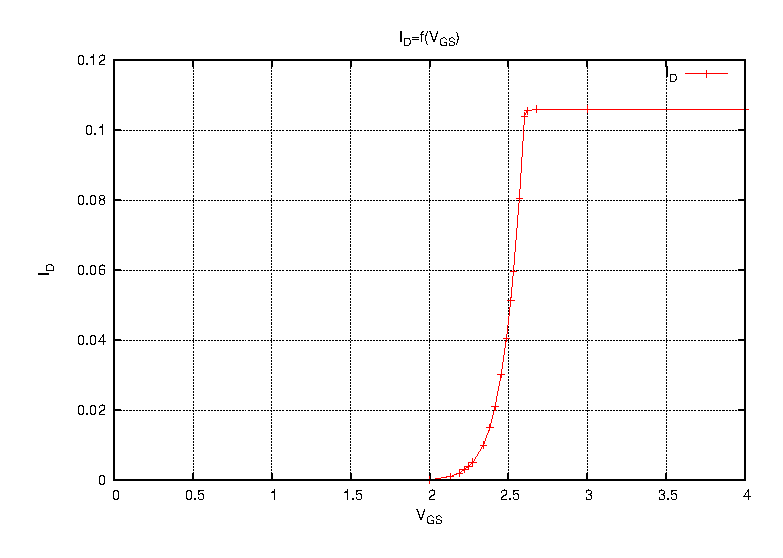
\includegraphics{id_vgs}}%
    \gplfronttext
  \end{picture}%
\endgroup
% GNUPLOT: LaTeX picture with Postscript
\begingroup
  \makeatletter
  \providecommand\color[2][]{%
    \GenericError{(gnuplot) \space\space\space\@spaces}{%
      Package color not loaded in conjunction with
      terminal option `colourtext'%
    }{See the gnuplot documentation for explanation.%
    }{Either use 'blacktext' in gnuplot or load the package
      color.sty in LaTeX.}%
    \renewcommand\color[2][]{}%
  }%
  \providecommand\includegraphics[2][]{%
    \GenericError{(gnuplot) \space\space\space\@spaces}{%
      Package graphicx or graphics not loaded%
    }{See the gnuplot documentation for explanation.%
    }{The gnuplot epslatex terminal needs graphicx.sty or graphics.sty.}%
    \renewcommand\includegraphics[2][]{}%
  }%
  \providecommand\rotatebox[2]{#2}%
  \@ifundefined{ifGPcolor}{%
    \newif\ifGPcolor
    \GPcolortrue
  }{}%
  \@ifundefined{ifGPblacktext}{%
    \newif\ifGPblacktext
    \GPblacktexttrue
  }{}%
  % define a \g@addto@macro without @ in the name:
  \let\gplgaddtomacro\g@addto@macro
  % define empty templates for all commands taking text:
  \gdef\gplbacktext{}%
  \gdef\gplfronttext{}%
  \makeatother
  \ifGPblacktext
    % no textcolor at all
    \def\colorrgb#1{}%
    \def\colorgray#1{}%
  \else
    % gray or color?
    \ifGPcolor
      \def\colorrgb#1{\color[rgb]{#1}}%
      \def\colorgray#1{\color[gray]{#1}}%
      \expandafter\def\csname LTw\endcsname{\color{white}}%
      \expandafter\def\csname LTb\endcsname{\color{black}}%
      \expandafter\def\csname LTa\endcsname{\color{black}}%
      \expandafter\def\csname LT0\endcsname{\color[rgb]{1,0,0}}%
      \expandafter\def\csname LT1\endcsname{\color[rgb]{0,1,0}}%
      \expandafter\def\csname LT2\endcsname{\color[rgb]{0,0,1}}%
      \expandafter\def\csname LT3\endcsname{\color[rgb]{1,0,1}}%
      \expandafter\def\csname LT4\endcsname{\color[rgb]{0,1,1}}%
      \expandafter\def\csname LT5\endcsname{\color[rgb]{1,1,0}}%
      \expandafter\def\csname LT6\endcsname{\color[rgb]{0,0,0}}%
      \expandafter\def\csname LT7\endcsname{\color[rgb]{1,0.3,0}}%
      \expandafter\def\csname LT8\endcsname{\color[rgb]{0.5,0.5,0.5}}%
    \else
      % gray
      \def\colorrgb#1{\color{black}}%
      \def\colorgray#1{\color[gray]{#1}}%
      \expandafter\def\csname LTw\endcsname{\color{white}}%
      \expandafter\def\csname LTb\endcsname{\color{black}}%
      \expandafter\def\csname LTa\endcsname{\color{black}}%
      \expandafter\def\csname LT0\endcsname{\color{black}}%
      \expandafter\def\csname LT1\endcsname{\color{black}}%
      \expandafter\def\csname LT2\endcsname{\color{black}}%
      \expandafter\def\csname LT3\endcsname{\color{black}}%
      \expandafter\def\csname LT4\endcsname{\color{black}}%
      \expandafter\def\csname LT5\endcsname{\color{black}}%
      \expandafter\def\csname LT6\endcsname{\color{black}}%
      \expandafter\def\csname LT7\endcsname{\color{black}}%
      \expandafter\def\csname LT8\endcsname{\color{black}}%
    \fi
  \fi
  \setlength{\unitlength}{0.0500bp}%
  \begin{picture}(7200.00,5040.00)%
    \gplgaddtomacro\gplbacktext{%
      \csname LTb\endcsname%
      \put(1342,704){\makebox(0,0)[r]{\strut{} 0}}%
      \csname LTb\endcsname%
      \put(1342,1317){\makebox(0,0)[r]{\strut{} 0.02}}%
      \csname LTb\endcsname%
      \put(1342,1929){\makebox(0,0)[r]{\strut{} 0.04}}%
      \csname LTb\endcsname%
      \put(1342,2542){\makebox(0,0)[r]{\strut{} 0.06}}%
      \csname LTb\endcsname%
      \put(1342,3155){\makebox(0,0)[r]{\strut{} 0.08}}%
      \csname LTb\endcsname%
      \put(1342,3767){\makebox(0,0)[r]{\strut{} 0.1}}%
      \csname LTb\endcsname%
      \put(1342,4380){\makebox(0,0)[r]{\strut{} 0.12}}%
      \csname LTb\endcsname%
      \put(1474,484){\makebox(0,0){\strut{} 0}}%
      \csname LTb\endcsname%
      \put(2373,484){\makebox(0,0){\strut{} 0.5}}%
      \csname LTb\endcsname%
      \put(3273,484){\makebox(0,0){\strut{} 1}}%
      \csname LTb\endcsname%
      \put(4172,484){\makebox(0,0){\strut{} 1.5}}%
      \csname LTb\endcsname%
      \put(5071,484){\makebox(0,0){\strut{} 2}}%
      \csname LTb\endcsname%
      \put(5971,484){\makebox(0,0){\strut{} 2.5}}%
      \csname LTb\endcsname%
      \put(6870,484){\makebox(0,0){\strut{} 3}}%
      \put(440,2542){\rotatebox{90}{\makebox(0,0){\strut{}I_D}}}%
      \put(4172,154){\makebox(0,0){\strut{}V_{GS}}}%
      \put(4172,4710){\makebox(0,0){\strut{}I_D=f(V_{GS})}}%
    }%
    \gplgaddtomacro\gplfronttext{%
      \csname LTb\endcsname%
      \put(5883,4207){\makebox(0,0)[r]{\strut{}I_D}}%
    }%
    \gplbacktext
    \put(0,0){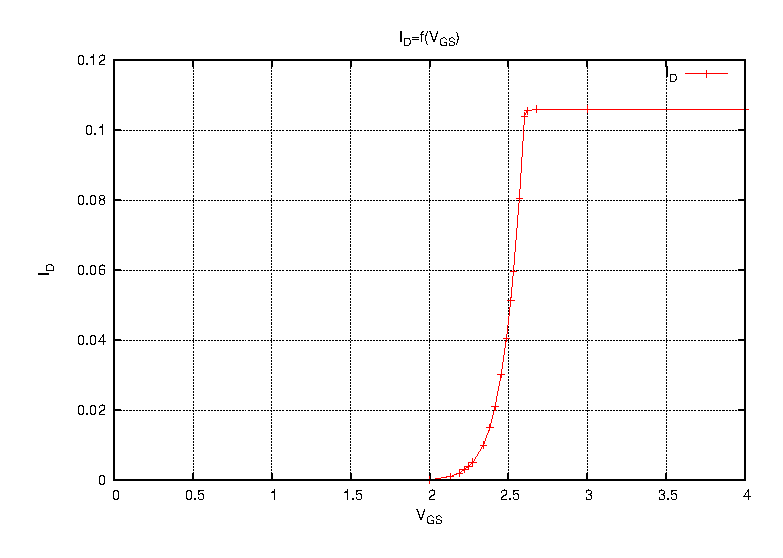
\includegraphics{id_vgs}}%
    \gplfronttext
  \end{picture}%
\endgroup
%!PS-Adobe-2.0
%%Title: id_vgs.tex
%%Creator: gnuplot 4.2 patchlevel 6 
%%CreationDate: Wed Dec 15 00:29:54 2010
%%DocumentFonts: (atend)
%%BoundingBox: 50 50 554 770
%%Orientation: Landscape
%%Pages: (atend)
%%EndComments
%%BeginProlog
/gnudict 256 dict def
gnudict begin
%
% The following 6 true/false flags may be edited by hand if required
% The unit line width may also be changed
%
/Color true def
/Blacktext false def
/Solid false def
/Dashlength 1 def
/Landscape true def
/Level1 false def
/Rounded false def
/TransparentPatterns false def
/gnulinewidth 5.000 def
/userlinewidth gnulinewidth def
%
/vshift -46 def
/dl1 {
  10.0 Dashlength mul mul
  Rounded { currentlinewidth 0.75 mul sub dup 0 le { pop 0.01 } if } if
} def
/dl2 {
  10.0 Dashlength mul mul
  Rounded { currentlinewidth 0.75 mul add } if
} def
/hpt_ 31.5 def
/vpt_ 31.5 def
/hpt hpt_ def
/vpt vpt_ def
Level1 {} {
/SDict 10 dict def
systemdict /pdfmark known not {
  userdict /pdfmark systemdict /cleartomark get put
} if
SDict begin [
  /Title (id_vgs.tex)
  /Subject (gnuplot plot)
  /Creator (gnuplot 4.2 patchlevel 6 )
  /Author (yallard)
%  /Producer (gnuplot)
%  /Keywords ()
  /CreationDate (Wed Dec 15 00:29:54 2010)
  /DOCINFO pdfmark
end
} ifelse
%
% Gnuplot Prolog Version 4.2 (August 2006)
%
/M {moveto} bind def
/L {lineto} bind def
/R {rmoveto} bind def
/V {rlineto} bind def
/N {newpath moveto} bind def
/Z {closepath} bind def
/C {setrgbcolor} bind def
/f {rlineto fill} bind def
/vpt2 vpt 2 mul def
/hpt2 hpt 2 mul def
/Lshow {currentpoint stroke M 0 vshift R 
	Blacktext {gsave 0 setgray show grestore} {show} ifelse} def
/Rshow {currentpoint stroke M dup stringwidth pop neg vshift R
	Blacktext {gsave 0 setgray show grestore} {show} ifelse} def
/Cshow {currentpoint stroke M dup stringwidth pop -2 div vshift R 
	Blacktext {gsave 0 setgray show grestore} {show} ifelse} def
/UP {dup vpt_ mul /vpt exch def hpt_ mul /hpt exch def
  /hpt2 hpt 2 mul def /vpt2 vpt 2 mul def} def
/DL {Color {setrgbcolor Solid {pop []} if 0 setdash}
 {pop pop pop 0 setgray Solid {pop []} if 0 setdash} ifelse} def
/BL {stroke userlinewidth 2 mul setlinewidth
	Rounded {1 setlinejoin 1 setlinecap} if} def
/AL {stroke userlinewidth 2 div setlinewidth
	Rounded {1 setlinejoin 1 setlinecap} if} def
/UL {dup gnulinewidth mul /userlinewidth exch def
	dup 1 lt {pop 1} if 10 mul /udl exch def} def
/PL {stroke userlinewidth setlinewidth
	Rounded {1 setlinejoin 1 setlinecap} if} def
% Default Line colors
/LCw {1 1 1} def
/LCb {0 0 0} def
/LCa {0 0 0} def
/LC0 {1 0 0} def
/LC1 {0 1 0} def
/LC2 {0 0 1} def
/LC3 {1 0 1} def
/LC4 {0 1 1} def
/LC5 {1 1 0} def
/LC6 {0 0 0} def
/LC7 {1 0.3 0} def
/LC8 {0.5 0.5 0.5} def
% Default Line Types
/LTw {PL [] 1 setgray} def
/LTb {BL [] LCb DL} def
/LTa {AL [1 udl mul 2 udl mul] 0 setdash LCa setrgbcolor} def
/LT0 {PL [] LC0 DL} def
/LT1 {PL [4 dl1 2 dl2] LC1 DL} def
/LT2 {PL [2 dl1 3 dl2] LC2 DL} def
/LT3 {PL [1 dl1 1.5 dl2] LC3 DL} def
/LT4 {PL [6 dl1 2 dl2 1 dl1 2 dl2] LC4 DL} def
/LT5 {PL [3 dl1 3 dl2 1 dl1 3 dl2] LC5 DL} def
/LT6 {PL [2 dl1 2 dl2 2 dl1 6 dl2] LC6 DL} def
/LT7 {PL [1 dl1 2 dl2 6 dl1 2 dl2 1 dl1 2 dl2] LC7 DL} def
/LT8 {PL [2 dl1 2 dl2 2 dl1 2 dl2 2 dl1 2 dl2 2 dl1 4 dl2] LC8 DL} def
/Pnt {stroke [] 0 setdash gsave 1 setlinecap M 0 0 V stroke grestore} def
/Dia {stroke [] 0 setdash 2 copy vpt add M
  hpt neg vpt neg V hpt vpt neg V
  hpt vpt V hpt neg vpt V closepath stroke
  Pnt} def
/Pls {stroke [] 0 setdash vpt sub M 0 vpt2 V
  currentpoint stroke M
  hpt neg vpt neg R hpt2 0 V stroke
 } def
/Box {stroke [] 0 setdash 2 copy exch hpt sub exch vpt add M
  0 vpt2 neg V hpt2 0 V 0 vpt2 V
  hpt2 neg 0 V closepath stroke
  Pnt} def
/Crs {stroke [] 0 setdash exch hpt sub exch vpt add M
  hpt2 vpt2 neg V currentpoint stroke M
  hpt2 neg 0 R hpt2 vpt2 V stroke} def
/TriU {stroke [] 0 setdash 2 copy vpt 1.12 mul add M
  hpt neg vpt -1.62 mul V
  hpt 2 mul 0 V
  hpt neg vpt 1.62 mul V closepath stroke
  Pnt} def
/Star {2 copy Pls Crs} def
/BoxF {stroke [] 0 setdash exch hpt sub exch vpt add M
  0 vpt2 neg V hpt2 0 V 0 vpt2 V
  hpt2 neg 0 V closepath fill} def
/TriUF {stroke [] 0 setdash vpt 1.12 mul add M
  hpt neg vpt -1.62 mul V
  hpt 2 mul 0 V
  hpt neg vpt 1.62 mul V closepath fill} def
/TriD {stroke [] 0 setdash 2 copy vpt 1.12 mul sub M
  hpt neg vpt 1.62 mul V
  hpt 2 mul 0 V
  hpt neg vpt -1.62 mul V closepath stroke
  Pnt} def
/TriDF {stroke [] 0 setdash vpt 1.12 mul sub M
  hpt neg vpt 1.62 mul V
  hpt 2 mul 0 V
  hpt neg vpt -1.62 mul V closepath fill} def
/DiaF {stroke [] 0 setdash vpt add M
  hpt neg vpt neg V hpt vpt neg V
  hpt vpt V hpt neg vpt V closepath fill} def
/Pent {stroke [] 0 setdash 2 copy gsave
  translate 0 hpt M 4 {72 rotate 0 hpt L} repeat
  closepath stroke grestore Pnt} def
/PentF {stroke [] 0 setdash gsave
  translate 0 hpt M 4 {72 rotate 0 hpt L} repeat
  closepath fill grestore} def
/Circle {stroke [] 0 setdash 2 copy
  hpt 0 360 arc stroke Pnt} def
/CircleF {stroke [] 0 setdash hpt 0 360 arc fill} def
/C0 {BL [] 0 setdash 2 copy moveto vpt 90 450 arc} bind def
/C1 {BL [] 0 setdash 2 copy moveto
	2 copy vpt 0 90 arc closepath fill
	vpt 0 360 arc closepath} bind def
/C2 {BL [] 0 setdash 2 copy moveto
	2 copy vpt 90 180 arc closepath fill
	vpt 0 360 arc closepath} bind def
/C3 {BL [] 0 setdash 2 copy moveto
	2 copy vpt 0 180 arc closepath fill
	vpt 0 360 arc closepath} bind def
/C4 {BL [] 0 setdash 2 copy moveto
	2 copy vpt 180 270 arc closepath fill
	vpt 0 360 arc closepath} bind def
/C5 {BL [] 0 setdash 2 copy moveto
	2 copy vpt 0 90 arc
	2 copy moveto
	2 copy vpt 180 270 arc closepath fill
	vpt 0 360 arc} bind def
/C6 {BL [] 0 setdash 2 copy moveto
	2 copy vpt 90 270 arc closepath fill
	vpt 0 360 arc closepath} bind def
/C7 {BL [] 0 setdash 2 copy moveto
	2 copy vpt 0 270 arc closepath fill
	vpt 0 360 arc closepath} bind def
/C8 {BL [] 0 setdash 2 copy moveto
	2 copy vpt 270 360 arc closepath fill
	vpt 0 360 arc closepath} bind def
/C9 {BL [] 0 setdash 2 copy moveto
	2 copy vpt 270 450 arc closepath fill
	vpt 0 360 arc closepath} bind def
/C10 {BL [] 0 setdash 2 copy 2 copy moveto vpt 270 360 arc closepath fill
	2 copy moveto
	2 copy vpt 90 180 arc closepath fill
	vpt 0 360 arc closepath} bind def
/C11 {BL [] 0 setdash 2 copy moveto
	2 copy vpt 0 180 arc closepath fill
	2 copy moveto
	2 copy vpt 270 360 arc closepath fill
	vpt 0 360 arc closepath} bind def
/C12 {BL [] 0 setdash 2 copy moveto
	2 copy vpt 180 360 arc closepath fill
	vpt 0 360 arc closepath} bind def
/C13 {BL [] 0 setdash 2 copy moveto
	2 copy vpt 0 90 arc closepath fill
	2 copy moveto
	2 copy vpt 180 360 arc closepath fill
	vpt 0 360 arc closepath} bind def
/C14 {BL [] 0 setdash 2 copy moveto
	2 copy vpt 90 360 arc closepath fill
	vpt 0 360 arc} bind def
/C15 {BL [] 0 setdash 2 copy vpt 0 360 arc closepath fill
	vpt 0 360 arc closepath} bind def
/Rec {newpath 4 2 roll moveto 1 index 0 rlineto 0 exch rlineto
	neg 0 rlineto closepath} bind def
/Square {dup Rec} bind def
/Bsquare {vpt sub exch vpt sub exch vpt2 Square} bind def
/S0 {BL [] 0 setdash 2 copy moveto 0 vpt rlineto BL Bsquare} bind def
/S1 {BL [] 0 setdash 2 copy vpt Square fill Bsquare} bind def
/S2 {BL [] 0 setdash 2 copy exch vpt sub exch vpt Square fill Bsquare} bind def
/S3 {BL [] 0 setdash 2 copy exch vpt sub exch vpt2 vpt Rec fill Bsquare} bind def
/S4 {BL [] 0 setdash 2 copy exch vpt sub exch vpt sub vpt Square fill Bsquare} bind def
/S5 {BL [] 0 setdash 2 copy 2 copy vpt Square fill
	exch vpt sub exch vpt sub vpt Square fill Bsquare} bind def
/S6 {BL [] 0 setdash 2 copy exch vpt sub exch vpt sub vpt vpt2 Rec fill Bsquare} bind def
/S7 {BL [] 0 setdash 2 copy exch vpt sub exch vpt sub vpt vpt2 Rec fill
	2 copy vpt Square fill Bsquare} bind def
/S8 {BL [] 0 setdash 2 copy vpt sub vpt Square fill Bsquare} bind def
/S9 {BL [] 0 setdash 2 copy vpt sub vpt vpt2 Rec fill Bsquare} bind def
/S10 {BL [] 0 setdash 2 copy vpt sub vpt Square fill 2 copy exch vpt sub exch vpt Square fill
	Bsquare} bind def
/S11 {BL [] 0 setdash 2 copy vpt sub vpt Square fill 2 copy exch vpt sub exch vpt2 vpt Rec fill
	Bsquare} bind def
/S12 {BL [] 0 setdash 2 copy exch vpt sub exch vpt sub vpt2 vpt Rec fill Bsquare} bind def
/S13 {BL [] 0 setdash 2 copy exch vpt sub exch vpt sub vpt2 vpt Rec fill
	2 copy vpt Square fill Bsquare} bind def
/S14 {BL [] 0 setdash 2 copy exch vpt sub exch vpt sub vpt2 vpt Rec fill
	2 copy exch vpt sub exch vpt Square fill Bsquare} bind def
/S15 {BL [] 0 setdash 2 copy Bsquare fill Bsquare} bind def
/D0 {gsave translate 45 rotate 0 0 S0 stroke grestore} bind def
/D1 {gsave translate 45 rotate 0 0 S1 stroke grestore} bind def
/D2 {gsave translate 45 rotate 0 0 S2 stroke grestore} bind def
/D3 {gsave translate 45 rotate 0 0 S3 stroke grestore} bind def
/D4 {gsave translate 45 rotate 0 0 S4 stroke grestore} bind def
/D5 {gsave translate 45 rotate 0 0 S5 stroke grestore} bind def
/D6 {gsave translate 45 rotate 0 0 S6 stroke grestore} bind def
/D7 {gsave translate 45 rotate 0 0 S7 stroke grestore} bind def
/D8 {gsave translate 45 rotate 0 0 S8 stroke grestore} bind def
/D9 {gsave translate 45 rotate 0 0 S9 stroke grestore} bind def
/D10 {gsave translate 45 rotate 0 0 S10 stroke grestore} bind def
/D11 {gsave translate 45 rotate 0 0 S11 stroke grestore} bind def
/D12 {gsave translate 45 rotate 0 0 S12 stroke grestore} bind def
/D13 {gsave translate 45 rotate 0 0 S13 stroke grestore} bind def
/D14 {gsave translate 45 rotate 0 0 S14 stroke grestore} bind def
/D15 {gsave translate 45 rotate 0 0 S15 stroke grestore} bind def
/DiaE {stroke [] 0 setdash vpt add M
  hpt neg vpt neg V hpt vpt neg V
  hpt vpt V hpt neg vpt V closepath stroke} def
/BoxE {stroke [] 0 setdash exch hpt sub exch vpt add M
  0 vpt2 neg V hpt2 0 V 0 vpt2 V
  hpt2 neg 0 V closepath stroke} def
/TriUE {stroke [] 0 setdash vpt 1.12 mul add M
  hpt neg vpt -1.62 mul V
  hpt 2 mul 0 V
  hpt neg vpt 1.62 mul V closepath stroke} def
/TriDE {stroke [] 0 setdash vpt 1.12 mul sub M
  hpt neg vpt 1.62 mul V
  hpt 2 mul 0 V
  hpt neg vpt -1.62 mul V closepath stroke} def
/PentE {stroke [] 0 setdash gsave
  translate 0 hpt M 4 {72 rotate 0 hpt L} repeat
  closepath stroke grestore} def
/CircE {stroke [] 0 setdash 
  hpt 0 360 arc stroke} def
/Opaque {gsave closepath 1 setgray fill grestore 0 setgray closepath} def
/DiaW {stroke [] 0 setdash vpt add M
  hpt neg vpt neg V hpt vpt neg V
  hpt vpt V hpt neg vpt V Opaque stroke} def
/BoxW {stroke [] 0 setdash exch hpt sub exch vpt add M
  0 vpt2 neg V hpt2 0 V 0 vpt2 V
  hpt2 neg 0 V Opaque stroke} def
/TriUW {stroke [] 0 setdash vpt 1.12 mul add M
  hpt neg vpt -1.62 mul V
  hpt 2 mul 0 V
  hpt neg vpt 1.62 mul V Opaque stroke} def
/TriDW {stroke [] 0 setdash vpt 1.12 mul sub M
  hpt neg vpt 1.62 mul V
  hpt 2 mul 0 V
  hpt neg vpt -1.62 mul V Opaque stroke} def
/PentW {stroke [] 0 setdash gsave
  translate 0 hpt M 4 {72 rotate 0 hpt L} repeat
  Opaque stroke grestore} def
/CircW {stroke [] 0 setdash 
  hpt 0 360 arc Opaque stroke} def
/BoxFill {gsave Rec 1 setgray fill grestore} def
/Density {
  /Fillden exch def
  currentrgbcolor
  /ColB exch def /ColG exch def /ColR exch def
  /ColR ColR Fillden mul Fillden sub 1 add def
  /ColG ColG Fillden mul Fillden sub 1 add def
  /ColB ColB Fillden mul Fillden sub 1 add def
  ColR ColG ColB setrgbcolor} def
/BoxColFill {gsave Rec PolyFill} def
/PolyFill {gsave Density fill grestore grestore} def
/h {rlineto rlineto rlineto gsave closepath fill grestore} bind def
%
% PostScript Level 1 Pattern Fill routine for rectangles
% Usage: x y w h s a XX PatternFill
%	x,y = lower left corner of box to be filled
%	w,h = width and height of box
%	  a = angle in degrees between lines and x-axis
%	 XX = 0/1 for no/yes cross-hatch
%
/PatternFill {gsave /PFa [ 9 2 roll ] def
  PFa 0 get PFa 2 get 2 div add PFa 1 get PFa 3 get 2 div add translate
  PFa 2 get -2 div PFa 3 get -2 div PFa 2 get PFa 3 get Rec
  gsave 1 setgray fill grestore clip
  currentlinewidth 0.5 mul setlinewidth
  /PFs PFa 2 get dup mul PFa 3 get dup mul add sqrt def
  0 0 M PFa 5 get rotate PFs -2 div dup translate
  0 1 PFs PFa 4 get div 1 add floor cvi
	{PFa 4 get mul 0 M 0 PFs V} for
  0 PFa 6 get ne {
	0 1 PFs PFa 4 get div 1 add floor cvi
	{PFa 4 get mul 0 2 1 roll M PFs 0 V} for
 } if
  stroke grestore} def
%
/languagelevel where
 {pop languagelevel} {1} ifelse
 2 lt
	{/InterpretLevel1 true def}
	{/InterpretLevel1 Level1 def}
 ifelse
%
% PostScript level 2 pattern fill definitions
%
/Level2PatternFill {
/Tile8x8 {/PaintType 2 /PatternType 1 /TilingType 1 /BBox [0 0 8 8] /XStep 8 /YStep 8}
	bind def
/KeepColor {currentrgbcolor [/Pattern /DeviceRGB] setcolorspace} bind def
<< Tile8x8
 /PaintProc {0.5 setlinewidth pop 0 0 M 8 8 L 0 8 M 8 0 L stroke} 
>> matrix makepattern
/Pat1 exch def
<< Tile8x8
 /PaintProc {0.5 setlinewidth pop 0 0 M 8 8 L 0 8 M 8 0 L stroke
	0 4 M 4 8 L 8 4 L 4 0 L 0 4 L stroke}
>> matrix makepattern
/Pat2 exch def
<< Tile8x8
 /PaintProc {0.5 setlinewidth pop 0 0 M 0 8 L
	8 8 L 8 0 L 0 0 L fill}
>> matrix makepattern
/Pat3 exch def
<< Tile8x8
 /PaintProc {0.5 setlinewidth pop -4 8 M 8 -4 L
	0 12 M 12 0 L stroke}
>> matrix makepattern
/Pat4 exch def
<< Tile8x8
 /PaintProc {0.5 setlinewidth pop -4 0 M 8 12 L
	0 -4 M 12 8 L stroke}
>> matrix makepattern
/Pat5 exch def
<< Tile8x8
 /PaintProc {0.5 setlinewidth pop -2 8 M 4 -4 L
	0 12 M 8 -4 L 4 12 M 10 0 L stroke}
>> matrix makepattern
/Pat6 exch def
<< Tile8x8
 /PaintProc {0.5 setlinewidth pop -2 0 M 4 12 L
	0 -4 M 8 12 L 4 -4 M 10 8 L stroke}
>> matrix makepattern
/Pat7 exch def
<< Tile8x8
 /PaintProc {0.5 setlinewidth pop 8 -2 M -4 4 L
	12 0 M -4 8 L 12 4 M 0 10 L stroke}
>> matrix makepattern
/Pat8 exch def
<< Tile8x8
 /PaintProc {0.5 setlinewidth pop 0 -2 M 12 4 L
	-4 0 M 12 8 L -4 4 M 8 10 L stroke}
>> matrix makepattern
/Pat9 exch def
/Pattern1 {PatternBgnd KeepColor Pat1 setpattern} bind def
/Pattern2 {PatternBgnd KeepColor Pat2 setpattern} bind def
/Pattern3 {PatternBgnd KeepColor Pat3 setpattern} bind def
/Pattern4 {PatternBgnd KeepColor Landscape {Pat5} {Pat4} ifelse setpattern} bind def
/Pattern5 {PatternBgnd KeepColor Landscape {Pat4} {Pat5} ifelse setpattern} bind def
/Pattern6 {PatternBgnd KeepColor Landscape {Pat9} {Pat6} ifelse setpattern} bind def
/Pattern7 {PatternBgnd KeepColor Landscape {Pat8} {Pat7} ifelse setpattern} bind def
} def
%
%
%End of PostScript Level 2 code
%
/PatternBgnd {
  TransparentPatterns {} {gsave 1 setgray fill grestore} ifelse
} def
%
% Substitute for Level 2 pattern fill codes with
% grayscale if Level 2 support is not selected.
%
/Level1PatternFill {
/Pattern1 {0.250 Density} bind def
/Pattern2 {0.500 Density} bind def
/Pattern3 {0.750 Density} bind def
/Pattern4 {0.125 Density} bind def
/Pattern5 {0.375 Density} bind def
/Pattern6 {0.625 Density} bind def
/Pattern7 {0.875 Density} bind def
} def
%
% Now test for support of Level 2 code
%
Level1 {Level1PatternFill} {Level2PatternFill} ifelse
%
/Symbol-Oblique /Symbol findfont [1 0 .167 1 0 0] makefont
dup length dict begin {1 index /FID eq {pop pop} {def} ifelse} forall
currentdict end definefont pop
/MFshow {
   { dup 5 get 3 ge
     { 5 get 3 eq {gsave} {grestore} ifelse }
     {dup dup 0 get findfont exch 1 get scalefont setfont
     [ currentpoint ] exch dup 2 get 0 exch R dup 5 get 2 ne {dup dup 6
     get exch 4 get {show} {stringwidth pop 0 R} ifelse }if dup 5 get 0 eq
     {dup 3 get {2 get neg 0 exch R pop} {pop aload pop M} ifelse} {dup 5
     get 1 eq {dup 2 get exch dup 3 get exch 6 get stringwidth pop -2 div
     dup 0 R} {dup 6 get stringwidth pop -2 div 0 R 6 get
     show 2 index {aload pop M neg 3 -1 roll neg R pop pop} {pop pop pop
     pop aload pop M} ifelse }ifelse }ifelse }
     ifelse }
   forall} bind def
/MFwidth {0 exch { dup 5 get 3 ge { 5 get 3 eq { 0 } { pop } ifelse }
 {dup 3 get{dup dup 0 get findfont exch 1 get scalefont setfont
     6 get stringwidth pop add} {pop} ifelse} ifelse} forall} bind def
/MLshow { currentpoint stroke M
  0 exch R
  Blacktext {gsave 0 setgray MFshow grestore} {MFshow} ifelse } bind def
/MRshow { currentpoint stroke M
  exch dup MFwidth neg 3 -1 roll R
  Blacktext {gsave 0 setgray MFshow grestore} {MFshow} ifelse } bind def
/MCshow { currentpoint stroke M
  exch dup MFwidth -2 div 3 -1 roll R
  Blacktext {gsave 0 setgray MFshow grestore} {MFshow} ifelse } bind def
/XYsave    { [( ) 1 2 true false 3 ()] } bind def
/XYrestore { [( ) 1 2 true false 4 ()] } bind def
end
%%EndProlog
%%Page: 1 1
gnudict begin
gsave
50 50 translate
0.100 0.100 scale
90 rotate
0 -5040 translate
0 setgray
newpath
(Helvetica) findfont 140 scalefont setfont
1.000 UL
LTb
1.000 UL
LTa
938 588 M
6052 0 V
stroke
LTb
938 588 M
63 0 V
5989 0 R
-63 0 V
stroke
854 588 M
[ [(Helvetica) 140.0 0.0 true true 0 ( 0)]
] -46.7 MRshow
1.000 UL
LTb
1.000 UL
LTa
938 1260 M
6052 0 V
stroke
LTb
938 1260 M
63 0 V
5989 0 R
-63 0 V
stroke
854 1260 M
[ [(Helvetica) 140.0 0.0 true true 0 ( 0.02)]
] -46.7 MRshow
1.000 UL
LTb
1.000 UL
LTa
938 1932 M
6052 0 V
stroke
LTb
938 1932 M
63 0 V
5989 0 R
-63 0 V
stroke
854 1932 M
[ [(Helvetica) 140.0 0.0 true true 0 ( 0.04)]
] -46.7 MRshow
1.000 UL
LTb
1.000 UL
LTa
938 2604 M
6052 0 V
stroke
LTb
938 2604 M
63 0 V
5989 0 R
-63 0 V
stroke
854 2604 M
[ [(Helvetica) 140.0 0.0 true true 0 ( 0.06)]
] -46.7 MRshow
1.000 UL
LTb
1.000 UL
LTa
938 3276 M
6052 0 V
stroke
LTb
938 3276 M
63 0 V
5989 0 R
-63 0 V
stroke
854 3276 M
[ [(Helvetica) 140.0 0.0 true true 0 ( 0.08)]
] -46.7 MRshow
1.000 UL
LTb
1.000 UL
LTa
938 3948 M
6052 0 V
stroke
LTb
938 3948 M
63 0 V
5989 0 R
-63 0 V
stroke
854 3948 M
[ [(Helvetica) 140.0 0.0 true true 0 ( 0.1)]
] -46.7 MRshow
1.000 UL
LTb
1.000 UL
LTa
938 4620 M
6052 0 V
stroke
LTb
938 4620 M
63 0 V
5989 0 R
-63 0 V
stroke
854 4620 M
[ [(Helvetica) 140.0 0.0 true true 0 ( 0.12)]
] -46.7 MRshow
1.000 UL
LTb
1.000 UL
LTa
938 588 M
0 4032 V
stroke
LTb
938 588 M
0 63 V
0 3969 R
0 -63 V
stroke
938 448 M
[ [(Helvetica) 140.0 0.0 true true 0 ( 0)]
] -46.7 MCshow
1.000 UL
LTb
1.000 UL
LTa
1947 588 M
0 4032 V
stroke
LTb
1947 588 M
0 63 V
0 3969 R
0 -63 V
stroke
1947 448 M
[ [(Helvetica) 140.0 0.0 true true 0 ( 0.5)]
] -46.7 MCshow
1.000 UL
LTb
1.000 UL
LTa
2955 588 M
0 4032 V
stroke
LTb
2955 588 M
0 63 V
0 3969 R
0 -63 V
stroke
2955 448 M
[ [(Helvetica) 140.0 0.0 true true 0 ( 1)]
] -46.7 MCshow
1.000 UL
LTb
1.000 UL
LTa
3964 588 M
0 4032 V
stroke
LTb
3964 588 M
0 63 V
0 3969 R
0 -63 V
stroke
3964 448 M
[ [(Helvetica) 140.0 0.0 true true 0 ( 1.5)]
] -46.7 MCshow
1.000 UL
LTb
1.000 UL
LTa
4973 588 M
0 4032 V
stroke
LTb
4973 588 M
0 63 V
0 3969 R
0 -63 V
stroke
4973 448 M
[ [(Helvetica) 140.0 0.0 true true 0 ( 2)]
] -46.7 MCshow
1.000 UL
LTb
1.000 UL
LTa
5981 588 M
0 4032 V
stroke
LTb
5981 588 M
0 63 V
0 3969 R
0 -63 V
stroke
5981 448 M
[ [(Helvetica) 140.0 0.0 true true 0 ( 2.5)]
] -46.7 MCshow
1.000 UL
LTb
1.000 UL
LTa
6990 588 M
0 4032 V
stroke
LTb
6990 588 M
0 63 V
0 3969 R
0 -63 V
stroke
6990 448 M
[ [(Helvetica) 140.0 0.0 true true 0 ( 3)]
] -46.7 MCshow
1.000 UL
LTb
1.000 UL
LTb
938 4620 N
938 588 L
6052 0 V
0 4032 V
-6052 0 V
Z stroke
LCb setrgbcolor
280 2604 M
currentpoint gsave translate 90 rotate 0 0 moveto
[ [(Helvetica) 140.0 0.0 true true 0 (I)]
[(Helvetica) 112.0 -42.0 true true 0 (D)]
] -32.7 MCshow
grestore
LTb
LCb setrgbcolor
3964 238 M
[ [(Helvetica) 140.0 0.0 true true 0 (V)]
[(Helvetica) 112.0 -42.0 true true 0 (GS)]
] -32.7 MCshow
LTb
3964 4830 M
[ [(Helvetica) 140.0 0.0 true true 0 (I)]
[(Helvetica) 112.0 -42.0 true true 0 (D)]
[(Helvetica) 140.0 0.0 true true 0 (=f\(V)]
[(Helvetica) 112.0 -42.0 true true 0 (GS)]
[(Helvetica) 140.0 0.0 true true 0 (\))]
] -32.7 MCshow
1.000 UP
1.000 UL
LTb
1.000 UP
1.000 UL
LT0
LTb
6339 4487 M
[ [(Helvetica) 140.0 0.0 true true 0 (I)]
[(Helvetica) 112.0 -42.0 true true 0 (D)]
] -32.7 MRshow
LT0
6423 4487 M
399 0 V
4973 589 M
262 33 V
121 33 V
60 34 V
61 33 V
50 37 V
136 165 V
80 168 V
67 198 V
81 316 V
66 343 V
55 359 V
34 283 V
77 702 V
66 789 V
4973 589 Pls
5235 622 Pls
5356 655 Pls
5416 689 Pls
5477 722 Pls
5527 759 Pls
5663 924 Pls
5743 1092 Pls
5810 1290 Pls
5891 1606 Pls
5957 1949 Pls
6012 2308 Pls
6046 2591 Pls
6123 3293 Pls
6189 4082 Pls
6622 4487 Pls
1.000 UL
LTb
938 4620 N
938 588 L
6052 0 V
0 4032 V
-6052 0 V
Z stroke
1.000 UP
1.000 UL
LTb
stroke
grestore
end
showpage
%%Trailer
%%DocumentFonts: Helvetica
%%Pages: 1
%!PS-Adobe-2.0 EPSF-2.0
%%Title: id_vgs.tex
%%Creator: gnuplot 4.2 patchlevel 6 
%%CreationDate: Wed Dec 15 00:31:15 2010
%%DocumentFonts: (atend)
%%BoundingBox: 50 50 410 302
%%EndComments
%%BeginProlog
/gnudict 256 dict def
gnudict begin
%
% The following 6 true/false flags may be edited by hand if required
% The unit line width may also be changed
%
/Color true def
/Blacktext false def
/Solid false def
/Dashlength 1 def
/Landscape false def
/Level1 false def
/Rounded false def
/TransparentPatterns false def
/gnulinewidth 5.000 def
/userlinewidth gnulinewidth def
%
/vshift -46 def
/dl1 {
  10.0 Dashlength mul mul
  Rounded { currentlinewidth 0.75 mul sub dup 0 le { pop 0.01 } if } if
} def
/dl2 {
  10.0 Dashlength mul mul
  Rounded { currentlinewidth 0.75 mul add } if
} def
/hpt_ 31.5 def
/vpt_ 31.5 def
/hpt hpt_ def
/vpt vpt_ def
Level1 {} {
/SDict 10 dict def
systemdict /pdfmark known not {
  userdict /pdfmark systemdict /cleartomark get put
} if
SDict begin [
  /Title (id_vgs.tex)
  /Subject (gnuplot plot)
  /Creator (gnuplot 4.2 patchlevel 6 )
  /Author (yallard)
%  /Producer (gnuplot)
%  /Keywords ()
  /CreationDate (Wed Dec 15 00:31:15 2010)
  /DOCINFO pdfmark
end
} ifelse
%
% Gnuplot Prolog Version 4.2 (August 2006)
%
/M {moveto} bind def
/L {lineto} bind def
/R {rmoveto} bind def
/V {rlineto} bind def
/N {newpath moveto} bind def
/Z {closepath} bind def
/C {setrgbcolor} bind def
/f {rlineto fill} bind def
/vpt2 vpt 2 mul def
/hpt2 hpt 2 mul def
/Lshow {currentpoint stroke M 0 vshift R 
	Blacktext {gsave 0 setgray show grestore} {show} ifelse} def
/Rshow {currentpoint stroke M dup stringwidth pop neg vshift R
	Blacktext {gsave 0 setgray show grestore} {show} ifelse} def
/Cshow {currentpoint stroke M dup stringwidth pop -2 div vshift R 
	Blacktext {gsave 0 setgray show grestore} {show} ifelse} def
/UP {dup vpt_ mul /vpt exch def hpt_ mul /hpt exch def
  /hpt2 hpt 2 mul def /vpt2 vpt 2 mul def} def
/DL {Color {setrgbcolor Solid {pop []} if 0 setdash}
 {pop pop pop 0 setgray Solid {pop []} if 0 setdash} ifelse} def
/BL {stroke userlinewidth 2 mul setlinewidth
	Rounded {1 setlinejoin 1 setlinecap} if} def
/AL {stroke userlinewidth 2 div setlinewidth
	Rounded {1 setlinejoin 1 setlinecap} if} def
/UL {dup gnulinewidth mul /userlinewidth exch def
	dup 1 lt {pop 1} if 10 mul /udl exch def} def
/PL {stroke userlinewidth setlinewidth
	Rounded {1 setlinejoin 1 setlinecap} if} def
% Default Line colors
/LCw {1 1 1} def
/LCb {0 0 0} def
/LCa {0 0 0} def
/LC0 {1 0 0} def
/LC1 {0 1 0} def
/LC2 {0 0 1} def
/LC3 {1 0 1} def
/LC4 {0 1 1} def
/LC5 {1 1 0} def
/LC6 {0 0 0} def
/LC7 {1 0.3 0} def
/LC8 {0.5 0.5 0.5} def
% Default Line Types
/LTw {PL [] 1 setgray} def
/LTb {BL [] LCb DL} def
/LTa {AL [1 udl mul 2 udl mul] 0 setdash LCa setrgbcolor} def
/LT0 {PL [] LC0 DL} def
/LT1 {PL [4 dl1 2 dl2] LC1 DL} def
/LT2 {PL [2 dl1 3 dl2] LC2 DL} def
/LT3 {PL [1 dl1 1.5 dl2] LC3 DL} def
/LT4 {PL [6 dl1 2 dl2 1 dl1 2 dl2] LC4 DL} def
/LT5 {PL [3 dl1 3 dl2 1 dl1 3 dl2] LC5 DL} def
/LT6 {PL [2 dl1 2 dl2 2 dl1 6 dl2] LC6 DL} def
/LT7 {PL [1 dl1 2 dl2 6 dl1 2 dl2 1 dl1 2 dl2] LC7 DL} def
/LT8 {PL [2 dl1 2 dl2 2 dl1 2 dl2 2 dl1 2 dl2 2 dl1 4 dl2] LC8 DL} def
/Pnt {stroke [] 0 setdash gsave 1 setlinecap M 0 0 V stroke grestore} def
/Dia {stroke [] 0 setdash 2 copy vpt add M
  hpt neg vpt neg V hpt vpt neg V
  hpt vpt V hpt neg vpt V closepath stroke
  Pnt} def
/Pls {stroke [] 0 setdash vpt sub M 0 vpt2 V
  currentpoint stroke M
  hpt neg vpt neg R hpt2 0 V stroke
 } def
/Box {stroke [] 0 setdash 2 copy exch hpt sub exch vpt add M
  0 vpt2 neg V hpt2 0 V 0 vpt2 V
  hpt2 neg 0 V closepath stroke
  Pnt} def
/Crs {stroke [] 0 setdash exch hpt sub exch vpt add M
  hpt2 vpt2 neg V currentpoint stroke M
  hpt2 neg 0 R hpt2 vpt2 V stroke} def
/TriU {stroke [] 0 setdash 2 copy vpt 1.12 mul add M
  hpt neg vpt -1.62 mul V
  hpt 2 mul 0 V
  hpt neg vpt 1.62 mul V closepath stroke
  Pnt} def
/Star {2 copy Pls Crs} def
/BoxF {stroke [] 0 setdash exch hpt sub exch vpt add M
  0 vpt2 neg V hpt2 0 V 0 vpt2 V
  hpt2 neg 0 V closepath fill} def
/TriUF {stroke [] 0 setdash vpt 1.12 mul add M
  hpt neg vpt -1.62 mul V
  hpt 2 mul 0 V
  hpt neg vpt 1.62 mul V closepath fill} def
/TriD {stroke [] 0 setdash 2 copy vpt 1.12 mul sub M
  hpt neg vpt 1.62 mul V
  hpt 2 mul 0 V
  hpt neg vpt -1.62 mul V closepath stroke
  Pnt} def
/TriDF {stroke [] 0 setdash vpt 1.12 mul sub M
  hpt neg vpt 1.62 mul V
  hpt 2 mul 0 V
  hpt neg vpt -1.62 mul V closepath fill} def
/DiaF {stroke [] 0 setdash vpt add M
  hpt neg vpt neg V hpt vpt neg V
  hpt vpt V hpt neg vpt V closepath fill} def
/Pent {stroke [] 0 setdash 2 copy gsave
  translate 0 hpt M 4 {72 rotate 0 hpt L} repeat
  closepath stroke grestore Pnt} def
/PentF {stroke [] 0 setdash gsave
  translate 0 hpt M 4 {72 rotate 0 hpt L} repeat
  closepath fill grestore} def
/Circle {stroke [] 0 setdash 2 copy
  hpt 0 360 arc stroke Pnt} def
/CircleF {stroke [] 0 setdash hpt 0 360 arc fill} def
/C0 {BL [] 0 setdash 2 copy moveto vpt 90 450 arc} bind def
/C1 {BL [] 0 setdash 2 copy moveto
	2 copy vpt 0 90 arc closepath fill
	vpt 0 360 arc closepath} bind def
/C2 {BL [] 0 setdash 2 copy moveto
	2 copy vpt 90 180 arc closepath fill
	vpt 0 360 arc closepath} bind def
/C3 {BL [] 0 setdash 2 copy moveto
	2 copy vpt 0 180 arc closepath fill
	vpt 0 360 arc closepath} bind def
/C4 {BL [] 0 setdash 2 copy moveto
	2 copy vpt 180 270 arc closepath fill
	vpt 0 360 arc closepath} bind def
/C5 {BL [] 0 setdash 2 copy moveto
	2 copy vpt 0 90 arc
	2 copy moveto
	2 copy vpt 180 270 arc closepath fill
	vpt 0 360 arc} bind def
/C6 {BL [] 0 setdash 2 copy moveto
	2 copy vpt 90 270 arc closepath fill
	vpt 0 360 arc closepath} bind def
/C7 {BL [] 0 setdash 2 copy moveto
	2 copy vpt 0 270 arc closepath fill
	vpt 0 360 arc closepath} bind def
/C8 {BL [] 0 setdash 2 copy moveto
	2 copy vpt 270 360 arc closepath fill
	vpt 0 360 arc closepath} bind def
/C9 {BL [] 0 setdash 2 copy moveto
	2 copy vpt 270 450 arc closepath fill
	vpt 0 360 arc closepath} bind def
/C10 {BL [] 0 setdash 2 copy 2 copy moveto vpt 270 360 arc closepath fill
	2 copy moveto
	2 copy vpt 90 180 arc closepath fill
	vpt 0 360 arc closepath} bind def
/C11 {BL [] 0 setdash 2 copy moveto
	2 copy vpt 0 180 arc closepath fill
	2 copy moveto
	2 copy vpt 270 360 arc closepath fill
	vpt 0 360 arc closepath} bind def
/C12 {BL [] 0 setdash 2 copy moveto
	2 copy vpt 180 360 arc closepath fill
	vpt 0 360 arc closepath} bind def
/C13 {BL [] 0 setdash 2 copy moveto
	2 copy vpt 0 90 arc closepath fill
	2 copy moveto
	2 copy vpt 180 360 arc closepath fill
	vpt 0 360 arc closepath} bind def
/C14 {BL [] 0 setdash 2 copy moveto
	2 copy vpt 90 360 arc closepath fill
	vpt 0 360 arc} bind def
/C15 {BL [] 0 setdash 2 copy vpt 0 360 arc closepath fill
	vpt 0 360 arc closepath} bind def
/Rec {newpath 4 2 roll moveto 1 index 0 rlineto 0 exch rlineto
	neg 0 rlineto closepath} bind def
/Square {dup Rec} bind def
/Bsquare {vpt sub exch vpt sub exch vpt2 Square} bind def
/S0 {BL [] 0 setdash 2 copy moveto 0 vpt rlineto BL Bsquare} bind def
/S1 {BL [] 0 setdash 2 copy vpt Square fill Bsquare} bind def
/S2 {BL [] 0 setdash 2 copy exch vpt sub exch vpt Square fill Bsquare} bind def
/S3 {BL [] 0 setdash 2 copy exch vpt sub exch vpt2 vpt Rec fill Bsquare} bind def
/S4 {BL [] 0 setdash 2 copy exch vpt sub exch vpt sub vpt Square fill Bsquare} bind def
/S5 {BL [] 0 setdash 2 copy 2 copy vpt Square fill
	exch vpt sub exch vpt sub vpt Square fill Bsquare} bind def
/S6 {BL [] 0 setdash 2 copy exch vpt sub exch vpt sub vpt vpt2 Rec fill Bsquare} bind def
/S7 {BL [] 0 setdash 2 copy exch vpt sub exch vpt sub vpt vpt2 Rec fill
	2 copy vpt Square fill Bsquare} bind def
/S8 {BL [] 0 setdash 2 copy vpt sub vpt Square fill Bsquare} bind def
/S9 {BL [] 0 setdash 2 copy vpt sub vpt vpt2 Rec fill Bsquare} bind def
/S10 {BL [] 0 setdash 2 copy vpt sub vpt Square fill 2 copy exch vpt sub exch vpt Square fill
	Bsquare} bind def
/S11 {BL [] 0 setdash 2 copy vpt sub vpt Square fill 2 copy exch vpt sub exch vpt2 vpt Rec fill
	Bsquare} bind def
/S12 {BL [] 0 setdash 2 copy exch vpt sub exch vpt sub vpt2 vpt Rec fill Bsquare} bind def
/S13 {BL [] 0 setdash 2 copy exch vpt sub exch vpt sub vpt2 vpt Rec fill
	2 copy vpt Square fill Bsquare} bind def
/S14 {BL [] 0 setdash 2 copy exch vpt sub exch vpt sub vpt2 vpt Rec fill
	2 copy exch vpt sub exch vpt Square fill Bsquare} bind def
/S15 {BL [] 0 setdash 2 copy Bsquare fill Bsquare} bind def
/D0 {gsave translate 45 rotate 0 0 S0 stroke grestore} bind def
/D1 {gsave translate 45 rotate 0 0 S1 stroke grestore} bind def
/D2 {gsave translate 45 rotate 0 0 S2 stroke grestore} bind def
/D3 {gsave translate 45 rotate 0 0 S3 stroke grestore} bind def
/D4 {gsave translate 45 rotate 0 0 S4 stroke grestore} bind def
/D5 {gsave translate 45 rotate 0 0 S5 stroke grestore} bind def
/D6 {gsave translate 45 rotate 0 0 S6 stroke grestore} bind def
/D7 {gsave translate 45 rotate 0 0 S7 stroke grestore} bind def
/D8 {gsave translate 45 rotate 0 0 S8 stroke grestore} bind def
/D9 {gsave translate 45 rotate 0 0 S9 stroke grestore} bind def
/D10 {gsave translate 45 rotate 0 0 S10 stroke grestore} bind def
/D11 {gsave translate 45 rotate 0 0 S11 stroke grestore} bind def
/D12 {gsave translate 45 rotate 0 0 S12 stroke grestore} bind def
/D13 {gsave translate 45 rotate 0 0 S13 stroke grestore} bind def
/D14 {gsave translate 45 rotate 0 0 S14 stroke grestore} bind def
/D15 {gsave translate 45 rotate 0 0 S15 stroke grestore} bind def
/DiaE {stroke [] 0 setdash vpt add M
  hpt neg vpt neg V hpt vpt neg V
  hpt vpt V hpt neg vpt V closepath stroke} def
/BoxE {stroke [] 0 setdash exch hpt sub exch vpt add M
  0 vpt2 neg V hpt2 0 V 0 vpt2 V
  hpt2 neg 0 V closepath stroke} def
/TriUE {stroke [] 0 setdash vpt 1.12 mul add M
  hpt neg vpt -1.62 mul V
  hpt 2 mul 0 V
  hpt neg vpt 1.62 mul V closepath stroke} def
/TriDE {stroke [] 0 setdash vpt 1.12 mul sub M
  hpt neg vpt 1.62 mul V
  hpt 2 mul 0 V
  hpt neg vpt -1.62 mul V closepath stroke} def
/PentE {stroke [] 0 setdash gsave
  translate 0 hpt M 4 {72 rotate 0 hpt L} repeat
  closepath stroke grestore} def
/CircE {stroke [] 0 setdash 
  hpt 0 360 arc stroke} def
/Opaque {gsave closepath 1 setgray fill grestore 0 setgray closepath} def
/DiaW {stroke [] 0 setdash vpt add M
  hpt neg vpt neg V hpt vpt neg V
  hpt vpt V hpt neg vpt V Opaque stroke} def
/BoxW {stroke [] 0 setdash exch hpt sub exch vpt add M
  0 vpt2 neg V hpt2 0 V 0 vpt2 V
  hpt2 neg 0 V Opaque stroke} def
/TriUW {stroke [] 0 setdash vpt 1.12 mul add M
  hpt neg vpt -1.62 mul V
  hpt 2 mul 0 V
  hpt neg vpt 1.62 mul V Opaque stroke} def
/TriDW {stroke [] 0 setdash vpt 1.12 mul sub M
  hpt neg vpt 1.62 mul V
  hpt 2 mul 0 V
  hpt neg vpt -1.62 mul V Opaque stroke} def
/PentW {stroke [] 0 setdash gsave
  translate 0 hpt M 4 {72 rotate 0 hpt L} repeat
  Opaque stroke grestore} def
/CircW {stroke [] 0 setdash 
  hpt 0 360 arc Opaque stroke} def
/BoxFill {gsave Rec 1 setgray fill grestore} def
/Density {
  /Fillden exch def
  currentrgbcolor
  /ColB exch def /ColG exch def /ColR exch def
  /ColR ColR Fillden mul Fillden sub 1 add def
  /ColG ColG Fillden mul Fillden sub 1 add def
  /ColB ColB Fillden mul Fillden sub 1 add def
  ColR ColG ColB setrgbcolor} def
/BoxColFill {gsave Rec PolyFill} def
/PolyFill {gsave Density fill grestore grestore} def
/h {rlineto rlineto rlineto gsave closepath fill grestore} bind def
%
% PostScript Level 1 Pattern Fill routine for rectangles
% Usage: x y w h s a XX PatternFill
%	x,y = lower left corner of box to be filled
%	w,h = width and height of box
%	  a = angle in degrees between lines and x-axis
%	 XX = 0/1 for no/yes cross-hatch
%
/PatternFill {gsave /PFa [ 9 2 roll ] def
  PFa 0 get PFa 2 get 2 div add PFa 1 get PFa 3 get 2 div add translate
  PFa 2 get -2 div PFa 3 get -2 div PFa 2 get PFa 3 get Rec
  gsave 1 setgray fill grestore clip
  currentlinewidth 0.5 mul setlinewidth
  /PFs PFa 2 get dup mul PFa 3 get dup mul add sqrt def
  0 0 M PFa 5 get rotate PFs -2 div dup translate
  0 1 PFs PFa 4 get div 1 add floor cvi
	{PFa 4 get mul 0 M 0 PFs V} for
  0 PFa 6 get ne {
	0 1 PFs PFa 4 get div 1 add floor cvi
	{PFa 4 get mul 0 2 1 roll M PFs 0 V} for
 } if
  stroke grestore} def
%
/languagelevel where
 {pop languagelevel} {1} ifelse
 2 lt
	{/InterpretLevel1 true def}
	{/InterpretLevel1 Level1 def}
 ifelse
%
% PostScript level 2 pattern fill definitions
%
/Level2PatternFill {
/Tile8x8 {/PaintType 2 /PatternType 1 /TilingType 1 /BBox [0 0 8 8] /XStep 8 /YStep 8}
	bind def
/KeepColor {currentrgbcolor [/Pattern /DeviceRGB] setcolorspace} bind def
<< Tile8x8
 /PaintProc {0.5 setlinewidth pop 0 0 M 8 8 L 0 8 M 8 0 L stroke} 
>> matrix makepattern
/Pat1 exch def
<< Tile8x8
 /PaintProc {0.5 setlinewidth pop 0 0 M 8 8 L 0 8 M 8 0 L stroke
	0 4 M 4 8 L 8 4 L 4 0 L 0 4 L stroke}
>> matrix makepattern
/Pat2 exch def
<< Tile8x8
 /PaintProc {0.5 setlinewidth pop 0 0 M 0 8 L
	8 8 L 8 0 L 0 0 L fill}
>> matrix makepattern
/Pat3 exch def
<< Tile8x8
 /PaintProc {0.5 setlinewidth pop -4 8 M 8 -4 L
	0 12 M 12 0 L stroke}
>> matrix makepattern
/Pat4 exch def
<< Tile8x8
 /PaintProc {0.5 setlinewidth pop -4 0 M 8 12 L
	0 -4 M 12 8 L stroke}
>> matrix makepattern
/Pat5 exch def
<< Tile8x8
 /PaintProc {0.5 setlinewidth pop -2 8 M 4 -4 L
	0 12 M 8 -4 L 4 12 M 10 0 L stroke}
>> matrix makepattern
/Pat6 exch def
<< Tile8x8
 /PaintProc {0.5 setlinewidth pop -2 0 M 4 12 L
	0 -4 M 8 12 L 4 -4 M 10 8 L stroke}
>> matrix makepattern
/Pat7 exch def
<< Tile8x8
 /PaintProc {0.5 setlinewidth pop 8 -2 M -4 4 L
	12 0 M -4 8 L 12 4 M 0 10 L stroke}
>> matrix makepattern
/Pat8 exch def
<< Tile8x8
 /PaintProc {0.5 setlinewidth pop 0 -2 M 12 4 L
	-4 0 M 12 8 L -4 4 M 8 10 L stroke}
>> matrix makepattern
/Pat9 exch def
/Pattern1 {PatternBgnd KeepColor Pat1 setpattern} bind def
/Pattern2 {PatternBgnd KeepColor Pat2 setpattern} bind def
/Pattern3 {PatternBgnd KeepColor Pat3 setpattern} bind def
/Pattern4 {PatternBgnd KeepColor Landscape {Pat5} {Pat4} ifelse setpattern} bind def
/Pattern5 {PatternBgnd KeepColor Landscape {Pat4} {Pat5} ifelse setpattern} bind def
/Pattern6 {PatternBgnd KeepColor Landscape {Pat9} {Pat6} ifelse setpattern} bind def
/Pattern7 {PatternBgnd KeepColor Landscape {Pat8} {Pat7} ifelse setpattern} bind def
} def
%
%
%End of PostScript Level 2 code
%
/PatternBgnd {
  TransparentPatterns {} {gsave 1 setgray fill grestore} ifelse
} def
%
% Substitute for Level 2 pattern fill codes with
% grayscale if Level 2 support is not selected.
%
/Level1PatternFill {
/Pattern1 {0.250 Density} bind def
/Pattern2 {0.500 Density} bind def
/Pattern3 {0.750 Density} bind def
/Pattern4 {0.125 Density} bind def
/Pattern5 {0.375 Density} bind def
/Pattern6 {0.625 Density} bind def
/Pattern7 {0.875 Density} bind def
} def
%
% Now test for support of Level 2 code
%
Level1 {Level1PatternFill} {Level2PatternFill} ifelse
%
/Symbol-Oblique /Symbol findfont [1 0 .167 1 0 0] makefont
dup length dict begin {1 index /FID eq {pop pop} {def} ifelse} forall
currentdict end definefont pop
/MFshow {
   { dup 5 get 3 ge
     { 5 get 3 eq {gsave} {grestore} ifelse }
     {dup dup 0 get findfont exch 1 get scalefont setfont
     [ currentpoint ] exch dup 2 get 0 exch R dup 5 get 2 ne {dup dup 6
     get exch 4 get {show} {stringwidth pop 0 R} ifelse }if dup 5 get 0 eq
     {dup 3 get {2 get neg 0 exch R pop} {pop aload pop M} ifelse} {dup 5
     get 1 eq {dup 2 get exch dup 3 get exch 6 get stringwidth pop -2 div
     dup 0 R} {dup 6 get stringwidth pop -2 div 0 R 6 get
     show 2 index {aload pop M neg 3 -1 roll neg R pop pop} {pop pop pop
     pop aload pop M} ifelse }ifelse }ifelse }
     ifelse }
   forall} bind def
/MFwidth {0 exch { dup 5 get 3 ge { 5 get 3 eq { 0 } { pop } ifelse }
 {dup 3 get{dup dup 0 get findfont exch 1 get scalefont setfont
     6 get stringwidth pop add} {pop} ifelse} ifelse} forall} bind def
/MLshow { currentpoint stroke M
  0 exch R
  Blacktext {gsave 0 setgray MFshow grestore} {MFshow} ifelse } bind def
/MRshow { currentpoint stroke M
  exch dup MFwidth neg 3 -1 roll R
  Blacktext {gsave 0 setgray MFshow grestore} {MFshow} ifelse } bind def
/MCshow { currentpoint stroke M
  exch dup MFwidth -2 div 3 -1 roll R
  Blacktext {gsave 0 setgray MFshow grestore} {MFshow} ifelse } bind def
/XYsave    { [( ) 1 2 true false 3 ()] } bind def
/XYrestore { [( ) 1 2 true false 4 ()] } bind def
end
%%EndProlog
gnudict begin
gsave
50 50 translate
0.050 0.050 scale
0 setgray
newpath
(Helvetica) findfont 140 scalefont setfont
1.000 UL
LTb
1.000 UL
LTa
938 588 M
6052 0 V
stroke
LTb
938 588 M
63 0 V
5989 0 R
-63 0 V
stroke
854 588 M
[ [(Helvetica) 140.0 0.0 true true 0 ( 0)]
] -46.7 MRshow
1.000 UL
LTb
1.000 UL
LTa
938 1260 M
6052 0 V
stroke
LTb
938 1260 M
63 0 V
5989 0 R
-63 0 V
stroke
854 1260 M
[ [(Helvetica) 140.0 0.0 true true 0 ( 0.02)]
] -46.7 MRshow
1.000 UL
LTb
1.000 UL
LTa
938 1932 M
6052 0 V
stroke
LTb
938 1932 M
63 0 V
5989 0 R
-63 0 V
stroke
854 1932 M
[ [(Helvetica) 140.0 0.0 true true 0 ( 0.04)]
] -46.7 MRshow
1.000 UL
LTb
1.000 UL
LTa
938 2604 M
6052 0 V
stroke
LTb
938 2604 M
63 0 V
5989 0 R
-63 0 V
stroke
854 2604 M
[ [(Helvetica) 140.0 0.0 true true 0 ( 0.06)]
] -46.7 MRshow
1.000 UL
LTb
1.000 UL
LTa
938 3276 M
6052 0 V
stroke
LTb
938 3276 M
63 0 V
5989 0 R
-63 0 V
stroke
854 3276 M
[ [(Helvetica) 140.0 0.0 true true 0 ( 0.08)]
] -46.7 MRshow
1.000 UL
LTb
1.000 UL
LTa
938 3948 M
6052 0 V
stroke
LTb
938 3948 M
63 0 V
5989 0 R
-63 0 V
stroke
854 3948 M
[ [(Helvetica) 140.0 0.0 true true 0 ( 0.1)]
] -46.7 MRshow
1.000 UL
LTb
1.000 UL
LTa
938 4620 M
6052 0 V
stroke
LTb
938 4620 M
63 0 V
5989 0 R
-63 0 V
stroke
854 4620 M
[ [(Helvetica) 140.0 0.0 true true 0 ( 0.12)]
] -46.7 MRshow
1.000 UL
LTb
1.000 UL
LTa
938 588 M
0 4032 V
stroke
LTb
938 588 M
0 63 V
0 3969 R
0 -63 V
stroke
938 448 M
[ [(Helvetica) 140.0 0.0 true true 0 ( 0)]
] -46.7 MCshow
1.000 UL
LTb
1.000 UL
LTa
1947 588 M
0 4032 V
stroke
LTb
1947 588 M
0 63 V
0 3969 R
0 -63 V
stroke
1947 448 M
[ [(Helvetica) 140.0 0.0 true true 0 ( 0.5)]
] -46.7 MCshow
1.000 UL
LTb
1.000 UL
LTa
2955 588 M
0 4032 V
stroke
LTb
2955 588 M
0 63 V
0 3969 R
0 -63 V
stroke
2955 448 M
[ [(Helvetica) 140.0 0.0 true true 0 ( 1)]
] -46.7 MCshow
1.000 UL
LTb
1.000 UL
LTa
3964 588 M
0 4032 V
stroke
LTb
3964 588 M
0 63 V
0 3969 R
0 -63 V
stroke
3964 448 M
[ [(Helvetica) 140.0 0.0 true true 0 ( 1.5)]
] -46.7 MCshow
1.000 UL
LTb
1.000 UL
LTa
4973 588 M
0 4032 V
stroke
LTb
4973 588 M
0 63 V
0 3969 R
0 -63 V
stroke
4973 448 M
[ [(Helvetica) 140.0 0.0 true true 0 ( 2)]
] -46.7 MCshow
1.000 UL
LTb
1.000 UL
LTa
5981 588 M
0 4032 V
stroke
LTb
5981 588 M
0 63 V
0 3969 R
0 -63 V
stroke
5981 448 M
[ [(Helvetica) 140.0 0.0 true true 0 ( 2.5)]
] -46.7 MCshow
1.000 UL
LTb
1.000 UL
LTa
6990 588 M
0 4032 V
stroke
LTb
6990 588 M
0 63 V
0 3969 R
0 -63 V
stroke
6990 448 M
[ [(Helvetica) 140.0 0.0 true true 0 ( 3)]
] -46.7 MCshow
1.000 UL
LTb
1.000 UL
LTb
938 4620 N
938 588 L
6052 0 V
0 4032 V
-6052 0 V
Z stroke
LCb setrgbcolor
280 2604 M
currentpoint gsave translate 90 rotate 0 0 moveto
[ [(Helvetica) 140.0 0.0 true true 0 (I)]
[(Helvetica) 112.0 -42.0 true true 0 (D)]
] -32.7 MCshow
grestore
LTb
LCb setrgbcolor
3964 238 M
[ [(Helvetica) 140.0 0.0 true true 0 (V)]
[(Helvetica) 112.0 -42.0 true true 0 (GS)]
] -32.7 MCshow
LTb
3964 4830 M
[ [(Helvetica) 140.0 0.0 true true 0 (I)]
[(Helvetica) 112.0 -42.0 true true 0 (D)]
[(Helvetica) 140.0 0.0 true true 0 (=f\(V)]
[(Helvetica) 112.0 -42.0 true true 0 (GS)]
[(Helvetica) 140.0 0.0 true true 0 (\))]
] -32.7 MCshow
1.000 UP
1.000 UL
LTb
1.000 UP
1.000 UL
LT0
LTb
6339 4487 M
[ [(Helvetica) 140.0 0.0 true true 0 (I)]
[(Helvetica) 112.0 -42.0 true true 0 (D)]
] -32.7 MRshow
LT0
6423 4487 M
399 0 V
4973 589 M
262 33 V
121 33 V
60 34 V
61 33 V
50 37 V
136 165 V
80 168 V
67 198 V
81 316 V
66 343 V
55 359 V
34 283 V
77 702 V
66 789 V
4973 589 Pls
5235 622 Pls
5356 655 Pls
5416 689 Pls
5477 722 Pls
5527 759 Pls
5663 924 Pls
5743 1092 Pls
5810 1290 Pls
5891 1606 Pls
5957 1949 Pls
6012 2308 Pls
6046 2591 Pls
6123 3293 Pls
6189 4082 Pls
6622 4487 Pls
1.000 UL
LTb
938 4620 N
938 588 L
6052 0 V
0 4032 V
-6052 0 V
Z stroke
1.000 UP
1.000 UL
LTb
stroke
grestore
end
showpage
%%Trailer
%%DocumentFonts: Helvetica
%!PS-Adobe-2.0 EPSF-2.0
%%Title: id_vgs.tex
%%Creator: gnuplot 4.2 patchlevel 6 
%%CreationDate: Wed Dec 15 00:31:44 2010
%%DocumentFonts: (atend)
%%BoundingBox: 50 50 410 302
%%EndComments
%%BeginProlog
/gnudict 256 dict def
gnudict begin
%
% The following 6 true/false flags may be edited by hand if required
% The unit line width may also be changed
%
/Color true def
/Blacktext false def
/Solid false def
/Dashlength 1 def
/Landscape false def
/Level1 false def
/Rounded false def
/TransparentPatterns false def
/gnulinewidth 5.000 def
/userlinewidth gnulinewidth def
%
/vshift -46 def
/dl1 {
  10.0 Dashlength mul mul
  Rounded { currentlinewidth 0.75 mul sub dup 0 le { pop 0.01 } if } if
} def
/dl2 {
  10.0 Dashlength mul mul
  Rounded { currentlinewidth 0.75 mul add } if
} def
/hpt_ 31.5 def
/vpt_ 31.5 def
/hpt hpt_ def
/vpt vpt_ def
Level1 {} {
/SDict 10 dict def
systemdict /pdfmark known not {
  userdict /pdfmark systemdict /cleartomark get put
} if
SDict begin [
  /Title (id_vgs.tex)
  /Subject (gnuplot plot)
  /Creator (gnuplot 4.2 patchlevel 6 )
  /Author (yallard)
%  /Producer (gnuplot)
%  /Keywords ()
  /CreationDate (Wed Dec 15 00:31:44 2010)
  /DOCINFO pdfmark
end
} ifelse
%
% Gnuplot Prolog Version 4.2 (August 2006)
%
/M {moveto} bind def
/L {lineto} bind def
/R {rmoveto} bind def
/V {rlineto} bind def
/N {newpath moveto} bind def
/Z {closepath} bind def
/C {setrgbcolor} bind def
/f {rlineto fill} bind def
/vpt2 vpt 2 mul def
/hpt2 hpt 2 mul def
/Lshow {currentpoint stroke M 0 vshift R 
	Blacktext {gsave 0 setgray show grestore} {show} ifelse} def
/Rshow {currentpoint stroke M dup stringwidth pop neg vshift R
	Blacktext {gsave 0 setgray show grestore} {show} ifelse} def
/Cshow {currentpoint stroke M dup stringwidth pop -2 div vshift R 
	Blacktext {gsave 0 setgray show grestore} {show} ifelse} def
/UP {dup vpt_ mul /vpt exch def hpt_ mul /hpt exch def
  /hpt2 hpt 2 mul def /vpt2 vpt 2 mul def} def
/DL {Color {setrgbcolor Solid {pop []} if 0 setdash}
 {pop pop pop 0 setgray Solid {pop []} if 0 setdash} ifelse} def
/BL {stroke userlinewidth 2 mul setlinewidth
	Rounded {1 setlinejoin 1 setlinecap} if} def
/AL {stroke userlinewidth 2 div setlinewidth
	Rounded {1 setlinejoin 1 setlinecap} if} def
/UL {dup gnulinewidth mul /userlinewidth exch def
	dup 1 lt {pop 1} if 10 mul /udl exch def} def
/PL {stroke userlinewidth setlinewidth
	Rounded {1 setlinejoin 1 setlinecap} if} def
% Default Line colors
/LCw {1 1 1} def
/LCb {0 0 0} def
/LCa {0 0 0} def
/LC0 {1 0 0} def
/LC1 {0 1 0} def
/LC2 {0 0 1} def
/LC3 {1 0 1} def
/LC4 {0 1 1} def
/LC5 {1 1 0} def
/LC6 {0 0 0} def
/LC7 {1 0.3 0} def
/LC8 {0.5 0.5 0.5} def
% Default Line Types
/LTw {PL [] 1 setgray} def
/LTb {BL [] LCb DL} def
/LTa {AL [1 udl mul 2 udl mul] 0 setdash LCa setrgbcolor} def
/LT0 {PL [] LC0 DL} def
/LT1 {PL [4 dl1 2 dl2] LC1 DL} def
/LT2 {PL [2 dl1 3 dl2] LC2 DL} def
/LT3 {PL [1 dl1 1.5 dl2] LC3 DL} def
/LT4 {PL [6 dl1 2 dl2 1 dl1 2 dl2] LC4 DL} def
/LT5 {PL [3 dl1 3 dl2 1 dl1 3 dl2] LC5 DL} def
/LT6 {PL [2 dl1 2 dl2 2 dl1 6 dl2] LC6 DL} def
/LT7 {PL [1 dl1 2 dl2 6 dl1 2 dl2 1 dl1 2 dl2] LC7 DL} def
/LT8 {PL [2 dl1 2 dl2 2 dl1 2 dl2 2 dl1 2 dl2 2 dl1 4 dl2] LC8 DL} def
/Pnt {stroke [] 0 setdash gsave 1 setlinecap M 0 0 V stroke grestore} def
/Dia {stroke [] 0 setdash 2 copy vpt add M
  hpt neg vpt neg V hpt vpt neg V
  hpt vpt V hpt neg vpt V closepath stroke
  Pnt} def
/Pls {stroke [] 0 setdash vpt sub M 0 vpt2 V
  currentpoint stroke M
  hpt neg vpt neg R hpt2 0 V stroke
 } def
/Box {stroke [] 0 setdash 2 copy exch hpt sub exch vpt add M
  0 vpt2 neg V hpt2 0 V 0 vpt2 V
  hpt2 neg 0 V closepath stroke
  Pnt} def
/Crs {stroke [] 0 setdash exch hpt sub exch vpt add M
  hpt2 vpt2 neg V currentpoint stroke M
  hpt2 neg 0 R hpt2 vpt2 V stroke} def
/TriU {stroke [] 0 setdash 2 copy vpt 1.12 mul add M
  hpt neg vpt -1.62 mul V
  hpt 2 mul 0 V
  hpt neg vpt 1.62 mul V closepath stroke
  Pnt} def
/Star {2 copy Pls Crs} def
/BoxF {stroke [] 0 setdash exch hpt sub exch vpt add M
  0 vpt2 neg V hpt2 0 V 0 vpt2 V
  hpt2 neg 0 V closepath fill} def
/TriUF {stroke [] 0 setdash vpt 1.12 mul add M
  hpt neg vpt -1.62 mul V
  hpt 2 mul 0 V
  hpt neg vpt 1.62 mul V closepath fill} def
/TriD {stroke [] 0 setdash 2 copy vpt 1.12 mul sub M
  hpt neg vpt 1.62 mul V
  hpt 2 mul 0 V
  hpt neg vpt -1.62 mul V closepath stroke
  Pnt} def
/TriDF {stroke [] 0 setdash vpt 1.12 mul sub M
  hpt neg vpt 1.62 mul V
  hpt 2 mul 0 V
  hpt neg vpt -1.62 mul V closepath fill} def
/DiaF {stroke [] 0 setdash vpt add M
  hpt neg vpt neg V hpt vpt neg V
  hpt vpt V hpt neg vpt V closepath fill} def
/Pent {stroke [] 0 setdash 2 copy gsave
  translate 0 hpt M 4 {72 rotate 0 hpt L} repeat
  closepath stroke grestore Pnt} def
/PentF {stroke [] 0 setdash gsave
  translate 0 hpt M 4 {72 rotate 0 hpt L} repeat
  closepath fill grestore} def
/Circle {stroke [] 0 setdash 2 copy
  hpt 0 360 arc stroke Pnt} def
/CircleF {stroke [] 0 setdash hpt 0 360 arc fill} def
/C0 {BL [] 0 setdash 2 copy moveto vpt 90 450 arc} bind def
/C1 {BL [] 0 setdash 2 copy moveto
	2 copy vpt 0 90 arc closepath fill
	vpt 0 360 arc closepath} bind def
/C2 {BL [] 0 setdash 2 copy moveto
	2 copy vpt 90 180 arc closepath fill
	vpt 0 360 arc closepath} bind def
/C3 {BL [] 0 setdash 2 copy moveto
	2 copy vpt 0 180 arc closepath fill
	vpt 0 360 arc closepath} bind def
/C4 {BL [] 0 setdash 2 copy moveto
	2 copy vpt 180 270 arc closepath fill
	vpt 0 360 arc closepath} bind def
/C5 {BL [] 0 setdash 2 copy moveto
	2 copy vpt 0 90 arc
	2 copy moveto
	2 copy vpt 180 270 arc closepath fill
	vpt 0 360 arc} bind def
/C6 {BL [] 0 setdash 2 copy moveto
	2 copy vpt 90 270 arc closepath fill
	vpt 0 360 arc closepath} bind def
/C7 {BL [] 0 setdash 2 copy moveto
	2 copy vpt 0 270 arc closepath fill
	vpt 0 360 arc closepath} bind def
/C8 {BL [] 0 setdash 2 copy moveto
	2 copy vpt 270 360 arc closepath fill
	vpt 0 360 arc closepath} bind def
/C9 {BL [] 0 setdash 2 copy moveto
	2 copy vpt 270 450 arc closepath fill
	vpt 0 360 arc closepath} bind def
/C10 {BL [] 0 setdash 2 copy 2 copy moveto vpt 270 360 arc closepath fill
	2 copy moveto
	2 copy vpt 90 180 arc closepath fill
	vpt 0 360 arc closepath} bind def
/C11 {BL [] 0 setdash 2 copy moveto
	2 copy vpt 0 180 arc closepath fill
	2 copy moveto
	2 copy vpt 270 360 arc closepath fill
	vpt 0 360 arc closepath} bind def
/C12 {BL [] 0 setdash 2 copy moveto
	2 copy vpt 180 360 arc closepath fill
	vpt 0 360 arc closepath} bind def
/C13 {BL [] 0 setdash 2 copy moveto
	2 copy vpt 0 90 arc closepath fill
	2 copy moveto
	2 copy vpt 180 360 arc closepath fill
	vpt 0 360 arc closepath} bind def
/C14 {BL [] 0 setdash 2 copy moveto
	2 copy vpt 90 360 arc closepath fill
	vpt 0 360 arc} bind def
/C15 {BL [] 0 setdash 2 copy vpt 0 360 arc closepath fill
	vpt 0 360 arc closepath} bind def
/Rec {newpath 4 2 roll moveto 1 index 0 rlineto 0 exch rlineto
	neg 0 rlineto closepath} bind def
/Square {dup Rec} bind def
/Bsquare {vpt sub exch vpt sub exch vpt2 Square} bind def
/S0 {BL [] 0 setdash 2 copy moveto 0 vpt rlineto BL Bsquare} bind def
/S1 {BL [] 0 setdash 2 copy vpt Square fill Bsquare} bind def
/S2 {BL [] 0 setdash 2 copy exch vpt sub exch vpt Square fill Bsquare} bind def
/S3 {BL [] 0 setdash 2 copy exch vpt sub exch vpt2 vpt Rec fill Bsquare} bind def
/S4 {BL [] 0 setdash 2 copy exch vpt sub exch vpt sub vpt Square fill Bsquare} bind def
/S5 {BL [] 0 setdash 2 copy 2 copy vpt Square fill
	exch vpt sub exch vpt sub vpt Square fill Bsquare} bind def
/S6 {BL [] 0 setdash 2 copy exch vpt sub exch vpt sub vpt vpt2 Rec fill Bsquare} bind def
/S7 {BL [] 0 setdash 2 copy exch vpt sub exch vpt sub vpt vpt2 Rec fill
	2 copy vpt Square fill Bsquare} bind def
/S8 {BL [] 0 setdash 2 copy vpt sub vpt Square fill Bsquare} bind def
/S9 {BL [] 0 setdash 2 copy vpt sub vpt vpt2 Rec fill Bsquare} bind def
/S10 {BL [] 0 setdash 2 copy vpt sub vpt Square fill 2 copy exch vpt sub exch vpt Square fill
	Bsquare} bind def
/S11 {BL [] 0 setdash 2 copy vpt sub vpt Square fill 2 copy exch vpt sub exch vpt2 vpt Rec fill
	Bsquare} bind def
/S12 {BL [] 0 setdash 2 copy exch vpt sub exch vpt sub vpt2 vpt Rec fill Bsquare} bind def
/S13 {BL [] 0 setdash 2 copy exch vpt sub exch vpt sub vpt2 vpt Rec fill
	2 copy vpt Square fill Bsquare} bind def
/S14 {BL [] 0 setdash 2 copy exch vpt sub exch vpt sub vpt2 vpt Rec fill
	2 copy exch vpt sub exch vpt Square fill Bsquare} bind def
/S15 {BL [] 0 setdash 2 copy Bsquare fill Bsquare} bind def
/D0 {gsave translate 45 rotate 0 0 S0 stroke grestore} bind def
/D1 {gsave translate 45 rotate 0 0 S1 stroke grestore} bind def
/D2 {gsave translate 45 rotate 0 0 S2 stroke grestore} bind def
/D3 {gsave translate 45 rotate 0 0 S3 stroke grestore} bind def
/D4 {gsave translate 45 rotate 0 0 S4 stroke grestore} bind def
/D5 {gsave translate 45 rotate 0 0 S5 stroke grestore} bind def
/D6 {gsave translate 45 rotate 0 0 S6 stroke grestore} bind def
/D7 {gsave translate 45 rotate 0 0 S7 stroke grestore} bind def
/D8 {gsave translate 45 rotate 0 0 S8 stroke grestore} bind def
/D9 {gsave translate 45 rotate 0 0 S9 stroke grestore} bind def
/D10 {gsave translate 45 rotate 0 0 S10 stroke grestore} bind def
/D11 {gsave translate 45 rotate 0 0 S11 stroke grestore} bind def
/D12 {gsave translate 45 rotate 0 0 S12 stroke grestore} bind def
/D13 {gsave translate 45 rotate 0 0 S13 stroke grestore} bind def
/D14 {gsave translate 45 rotate 0 0 S14 stroke grestore} bind def
/D15 {gsave translate 45 rotate 0 0 S15 stroke grestore} bind def
/DiaE {stroke [] 0 setdash vpt add M
  hpt neg vpt neg V hpt vpt neg V
  hpt vpt V hpt neg vpt V closepath stroke} def
/BoxE {stroke [] 0 setdash exch hpt sub exch vpt add M
  0 vpt2 neg V hpt2 0 V 0 vpt2 V
  hpt2 neg 0 V closepath stroke} def
/TriUE {stroke [] 0 setdash vpt 1.12 mul add M
  hpt neg vpt -1.62 mul V
  hpt 2 mul 0 V
  hpt neg vpt 1.62 mul V closepath stroke} def
/TriDE {stroke [] 0 setdash vpt 1.12 mul sub M
  hpt neg vpt 1.62 mul V
  hpt 2 mul 0 V
  hpt neg vpt -1.62 mul V closepath stroke} def
/PentE {stroke [] 0 setdash gsave
  translate 0 hpt M 4 {72 rotate 0 hpt L} repeat
  closepath stroke grestore} def
/CircE {stroke [] 0 setdash 
  hpt 0 360 arc stroke} def
/Opaque {gsave closepath 1 setgray fill grestore 0 setgray closepath} def
/DiaW {stroke [] 0 setdash vpt add M
  hpt neg vpt neg V hpt vpt neg V
  hpt vpt V hpt neg vpt V Opaque stroke} def
/BoxW {stroke [] 0 setdash exch hpt sub exch vpt add M
  0 vpt2 neg V hpt2 0 V 0 vpt2 V
  hpt2 neg 0 V Opaque stroke} def
/TriUW {stroke [] 0 setdash vpt 1.12 mul add M
  hpt neg vpt -1.62 mul V
  hpt 2 mul 0 V
  hpt neg vpt 1.62 mul V Opaque stroke} def
/TriDW {stroke [] 0 setdash vpt 1.12 mul sub M
  hpt neg vpt 1.62 mul V
  hpt 2 mul 0 V
  hpt neg vpt -1.62 mul V Opaque stroke} def
/PentW {stroke [] 0 setdash gsave
  translate 0 hpt M 4 {72 rotate 0 hpt L} repeat
  Opaque stroke grestore} def
/CircW {stroke [] 0 setdash 
  hpt 0 360 arc Opaque stroke} def
/BoxFill {gsave Rec 1 setgray fill grestore} def
/Density {
  /Fillden exch def
  currentrgbcolor
  /ColB exch def /ColG exch def /ColR exch def
  /ColR ColR Fillden mul Fillden sub 1 add def
  /ColG ColG Fillden mul Fillden sub 1 add def
  /ColB ColB Fillden mul Fillden sub 1 add def
  ColR ColG ColB setrgbcolor} def
/BoxColFill {gsave Rec PolyFill} def
/PolyFill {gsave Density fill grestore grestore} def
/h {rlineto rlineto rlineto gsave closepath fill grestore} bind def
%
% PostScript Level 1 Pattern Fill routine for rectangles
% Usage: x y w h s a XX PatternFill
%	x,y = lower left corner of box to be filled
%	w,h = width and height of box
%	  a = angle in degrees between lines and x-axis
%	 XX = 0/1 for no/yes cross-hatch
%
/PatternFill {gsave /PFa [ 9 2 roll ] def
  PFa 0 get PFa 2 get 2 div add PFa 1 get PFa 3 get 2 div add translate
  PFa 2 get -2 div PFa 3 get -2 div PFa 2 get PFa 3 get Rec
  gsave 1 setgray fill grestore clip
  currentlinewidth 0.5 mul setlinewidth
  /PFs PFa 2 get dup mul PFa 3 get dup mul add sqrt def
  0 0 M PFa 5 get rotate PFs -2 div dup translate
  0 1 PFs PFa 4 get div 1 add floor cvi
	{PFa 4 get mul 0 M 0 PFs V} for
  0 PFa 6 get ne {
	0 1 PFs PFa 4 get div 1 add floor cvi
	{PFa 4 get mul 0 2 1 roll M PFs 0 V} for
 } if
  stroke grestore} def
%
/languagelevel where
 {pop languagelevel} {1} ifelse
 2 lt
	{/InterpretLevel1 true def}
	{/InterpretLevel1 Level1 def}
 ifelse
%
% PostScript level 2 pattern fill definitions
%
/Level2PatternFill {
/Tile8x8 {/PaintType 2 /PatternType 1 /TilingType 1 /BBox [0 0 8 8] /XStep 8 /YStep 8}
	bind def
/KeepColor {currentrgbcolor [/Pattern /DeviceRGB] setcolorspace} bind def
<< Tile8x8
 /PaintProc {0.5 setlinewidth pop 0 0 M 8 8 L 0 8 M 8 0 L stroke} 
>> matrix makepattern
/Pat1 exch def
<< Tile8x8
 /PaintProc {0.5 setlinewidth pop 0 0 M 8 8 L 0 8 M 8 0 L stroke
	0 4 M 4 8 L 8 4 L 4 0 L 0 4 L stroke}
>> matrix makepattern
/Pat2 exch def
<< Tile8x8
 /PaintProc {0.5 setlinewidth pop 0 0 M 0 8 L
	8 8 L 8 0 L 0 0 L fill}
>> matrix makepattern
/Pat3 exch def
<< Tile8x8
 /PaintProc {0.5 setlinewidth pop -4 8 M 8 -4 L
	0 12 M 12 0 L stroke}
>> matrix makepattern
/Pat4 exch def
<< Tile8x8
 /PaintProc {0.5 setlinewidth pop -4 0 M 8 12 L
	0 -4 M 12 8 L stroke}
>> matrix makepattern
/Pat5 exch def
<< Tile8x8
 /PaintProc {0.5 setlinewidth pop -2 8 M 4 -4 L
	0 12 M 8 -4 L 4 12 M 10 0 L stroke}
>> matrix makepattern
/Pat6 exch def
<< Tile8x8
 /PaintProc {0.5 setlinewidth pop -2 0 M 4 12 L
	0 -4 M 8 12 L 4 -4 M 10 8 L stroke}
>> matrix makepattern
/Pat7 exch def
<< Tile8x8
 /PaintProc {0.5 setlinewidth pop 8 -2 M -4 4 L
	12 0 M -4 8 L 12 4 M 0 10 L stroke}
>> matrix makepattern
/Pat8 exch def
<< Tile8x8
 /PaintProc {0.5 setlinewidth pop 0 -2 M 12 4 L
	-4 0 M 12 8 L -4 4 M 8 10 L stroke}
>> matrix makepattern
/Pat9 exch def
/Pattern1 {PatternBgnd KeepColor Pat1 setpattern} bind def
/Pattern2 {PatternBgnd KeepColor Pat2 setpattern} bind def
/Pattern3 {PatternBgnd KeepColor Pat3 setpattern} bind def
/Pattern4 {PatternBgnd KeepColor Landscape {Pat5} {Pat4} ifelse setpattern} bind def
/Pattern5 {PatternBgnd KeepColor Landscape {Pat4} {Pat5} ifelse setpattern} bind def
/Pattern6 {PatternBgnd KeepColor Landscape {Pat9} {Pat6} ifelse setpattern} bind def
/Pattern7 {PatternBgnd KeepColor Landscape {Pat8} {Pat7} ifelse setpattern} bind def
} def
%
%
%End of PostScript Level 2 code
%
/PatternBgnd {
  TransparentPatterns {} {gsave 1 setgray fill grestore} ifelse
} def
%
% Substitute for Level 2 pattern fill codes with
% grayscale if Level 2 support is not selected.
%
/Level1PatternFill {
/Pattern1 {0.250 Density} bind def
/Pattern2 {0.500 Density} bind def
/Pattern3 {0.750 Density} bind def
/Pattern4 {0.125 Density} bind def
/Pattern5 {0.375 Density} bind def
/Pattern6 {0.625 Density} bind def
/Pattern7 {0.875 Density} bind def
} def
%
% Now test for support of Level 2 code
%
Level1 {Level1PatternFill} {Level2PatternFill} ifelse
%
/Symbol-Oblique /Symbol findfont [1 0 .167 1 0 0] makefont
dup length dict begin {1 index /FID eq {pop pop} {def} ifelse} forall
currentdict end definefont pop
/MFshow {
   { dup 5 get 3 ge
     { 5 get 3 eq {gsave} {grestore} ifelse }
     {dup dup 0 get findfont exch 1 get scalefont setfont
     [ currentpoint ] exch dup 2 get 0 exch R dup 5 get 2 ne {dup dup 6
     get exch 4 get {show} {stringwidth pop 0 R} ifelse }if dup 5 get 0 eq
     {dup 3 get {2 get neg 0 exch R pop} {pop aload pop M} ifelse} {dup 5
     get 1 eq {dup 2 get exch dup 3 get exch 6 get stringwidth pop -2 div
     dup 0 R} {dup 6 get stringwidth pop -2 div 0 R 6 get
     show 2 index {aload pop M neg 3 -1 roll neg R pop pop} {pop pop pop
     pop aload pop M} ifelse }ifelse }ifelse }
     ifelse }
   forall} bind def
/MFwidth {0 exch { dup 5 get 3 ge { 5 get 3 eq { 0 } { pop } ifelse }
 {dup 3 get{dup dup 0 get findfont exch 1 get scalefont setfont
     6 get stringwidth pop add} {pop} ifelse} ifelse} forall} bind def
/MLshow { currentpoint stroke M
  0 exch R
  Blacktext {gsave 0 setgray MFshow grestore} {MFshow} ifelse } bind def
/MRshow { currentpoint stroke M
  exch dup MFwidth neg 3 -1 roll R
  Blacktext {gsave 0 setgray MFshow grestore} {MFshow} ifelse } bind def
/MCshow { currentpoint stroke M
  exch dup MFwidth -2 div 3 -1 roll R
  Blacktext {gsave 0 setgray MFshow grestore} {MFshow} ifelse } bind def
/XYsave    { [( ) 1 2 true false 3 ()] } bind def
/XYrestore { [( ) 1 2 true false 4 ()] } bind def
end
%%EndProlog
gnudict begin
gsave
50 50 translate
0.050 0.050 scale
0 setgray
newpath
(Helvetica) findfont 140 scalefont setfont
1.000 UL
LTb
1.000 UL
LTa
938 588 M
6052 0 V
stroke
LTb
938 588 M
63 0 V
5989 0 R
-63 0 V
stroke
854 588 M
[ [(Helvetica) 140.0 0.0 true true 0 ( 0)]
] -46.7 MRshow
1.000 UL
LTb
1.000 UL
LTa
938 1260 M
6052 0 V
stroke
LTb
938 1260 M
63 0 V
5989 0 R
-63 0 V
stroke
854 1260 M
[ [(Helvetica) 140.0 0.0 true true 0 ( 0.02)]
] -46.7 MRshow
1.000 UL
LTb
1.000 UL
LTa
938 1932 M
6052 0 V
stroke
LTb
938 1932 M
63 0 V
5989 0 R
-63 0 V
stroke
854 1932 M
[ [(Helvetica) 140.0 0.0 true true 0 ( 0.04)]
] -46.7 MRshow
1.000 UL
LTb
1.000 UL
LTa
938 2604 M
6052 0 V
stroke
LTb
938 2604 M
63 0 V
5989 0 R
-63 0 V
stroke
854 2604 M
[ [(Helvetica) 140.0 0.0 true true 0 ( 0.06)]
] -46.7 MRshow
1.000 UL
LTb
1.000 UL
LTa
938 3276 M
6052 0 V
stroke
LTb
938 3276 M
63 0 V
5989 0 R
-63 0 V
stroke
854 3276 M
[ [(Helvetica) 140.0 0.0 true true 0 ( 0.08)]
] -46.7 MRshow
1.000 UL
LTb
1.000 UL
LTa
938 3948 M
6052 0 V
stroke
LTb
938 3948 M
63 0 V
5989 0 R
-63 0 V
stroke
854 3948 M
[ [(Helvetica) 140.0 0.0 true true 0 ( 0.1)]
] -46.7 MRshow
1.000 UL
LTb
1.000 UL
LTa
938 4620 M
6052 0 V
stroke
LTb
938 4620 M
63 0 V
5989 0 R
-63 0 V
stroke
854 4620 M
[ [(Helvetica) 140.0 0.0 true true 0 ( 0.12)]
] -46.7 MRshow
1.000 UL
LTb
1.000 UL
LTa
938 588 M
0 4032 V
stroke
LTb
938 588 M
0 63 V
0 3969 R
0 -63 V
stroke
938 448 M
[ [(Helvetica) 140.0 0.0 true true 0 ( 0)]
] -46.7 MCshow
1.000 UL
LTb
1.000 UL
LTa
1947 588 M
0 4032 V
stroke
LTb
1947 588 M
0 63 V
0 3969 R
0 -63 V
stroke
1947 448 M
[ [(Helvetica) 140.0 0.0 true true 0 ( 0.5)]
] -46.7 MCshow
1.000 UL
LTb
1.000 UL
LTa
2955 588 M
0 4032 V
stroke
LTb
2955 588 M
0 63 V
0 3969 R
0 -63 V
stroke
2955 448 M
[ [(Helvetica) 140.0 0.0 true true 0 ( 1)]
] -46.7 MCshow
1.000 UL
LTb
1.000 UL
LTa
3964 588 M
0 4032 V
stroke
LTb
3964 588 M
0 63 V
0 3969 R
0 -63 V
stroke
3964 448 M
[ [(Helvetica) 140.0 0.0 true true 0 ( 1.5)]
] -46.7 MCshow
1.000 UL
LTb
1.000 UL
LTa
4973 588 M
0 4032 V
stroke
LTb
4973 588 M
0 63 V
0 3969 R
0 -63 V
stroke
4973 448 M
[ [(Helvetica) 140.0 0.0 true true 0 ( 2)]
] -46.7 MCshow
1.000 UL
LTb
1.000 UL
LTa
5981 588 M
0 4032 V
stroke
LTb
5981 588 M
0 63 V
0 3969 R
0 -63 V
stroke
5981 448 M
[ [(Helvetica) 140.0 0.0 true true 0 ( 2.5)]
] -46.7 MCshow
1.000 UL
LTb
1.000 UL
LTa
6990 588 M
0 4032 V
stroke
LTb
6990 588 M
0 63 V
0 3969 R
0 -63 V
stroke
6990 448 M
[ [(Helvetica) 140.0 0.0 true true 0 ( 3)]
] -46.7 MCshow
1.000 UL
LTb
1.000 UL
LTb
938 4620 N
938 588 L
6052 0 V
0 4032 V
-6052 0 V
Z stroke
LCb setrgbcolor
280 2604 M
currentpoint gsave translate 90 rotate 0 0 moveto
[ [(Helvetica) 140.0 0.0 true true 0 (I)]
[(Helvetica) 112.0 -42.0 true true 0 (D)]
] -32.7 MCshow
grestore
LTb
LCb setrgbcolor
3964 238 M
[ [(Helvetica) 140.0 0.0 true true 0 (V)]
[(Helvetica) 112.0 -42.0 true true 0 (GS)]
] -32.7 MCshow
LTb
3964 4830 M
[ [(Helvetica) 140.0 0.0 true true 0 (I)]
[(Helvetica) 112.0 -42.0 true true 0 (D)]
[(Helvetica) 140.0 0.0 true true 0 (=f\(V)]
[(Helvetica) 112.0 -42.0 true true 0 (GS)]
[(Helvetica) 140.0 0.0 true true 0 (\))]
] -32.7 MCshow
1.000 UP
1.000 UL
LTb
1.000 UP
1.000 UL
LT0
LTb
6339 4487 M
[ [(Helvetica) 140.0 0.0 true true 0 (I)]
[(Helvetica) 112.0 -42.0 true true 0 (D)]
] -32.7 MRshow
LT0
6423 4487 M
399 0 V
4973 589 M
262 33 V
121 33 V
60 34 V
61 33 V
50 37 V
136 165 V
80 168 V
67 198 V
81 316 V
66 343 V
55 359 V
34 283 V
77 702 V
66 789 V
4973 589 Pls
5235 622 Pls
5356 655 Pls
5416 689 Pls
5477 722 Pls
5527 759 Pls
5663 924 Pls
5743 1092 Pls
5810 1290 Pls
5891 1606 Pls
5957 1949 Pls
6012 2308 Pls
6046 2591 Pls
6123 3293 Pls
6189 4082 Pls
6622 4487 Pls
1.000 UL
LTb
938 4620 N
938 588 L
6052 0 V
0 4032 V
-6052 0 V
Z stroke
1.000 UP
1.000 UL
LTb
stroke
grestore
end
showpage
gnudict begin
gsave
50 50 translate
0.050 0.050 scale
0 setgray
newpath
(Helvetica) findfont 140 scalefont setfont
1.000 UL
LTb
1.000 UL
LTa
938 588 M
6052 0 V
stroke
LTb
938 588 M
63 0 V
5989 0 R
-63 0 V
stroke
854 588 M
[ [(Helvetica) 140.0 0.0 true true 0 ( 0)]
] -46.7 MRshow
1.000 UL
LTb
1.000 UL
LTa
938 1260 M
6052 0 V
stroke
LTb
938 1260 M
63 0 V
5989 0 R
-63 0 V
stroke
854 1260 M
[ [(Helvetica) 140.0 0.0 true true 0 ( 0.02)]
] -46.7 MRshow
1.000 UL
LTb
1.000 UL
LTa
938 1932 M
6052 0 V
stroke
LTb
938 1932 M
63 0 V
5989 0 R
-63 0 V
stroke
854 1932 M
[ [(Helvetica) 140.0 0.0 true true 0 ( 0.04)]
] -46.7 MRshow
1.000 UL
LTb
1.000 UL
LTa
938 2604 M
6052 0 V
stroke
LTb
938 2604 M
63 0 V
5989 0 R
-63 0 V
stroke
854 2604 M
[ [(Helvetica) 140.0 0.0 true true 0 ( 0.06)]
] -46.7 MRshow
1.000 UL
LTb
1.000 UL
LTa
938 3276 M
6052 0 V
stroke
LTb
938 3276 M
63 0 V
5989 0 R
-63 0 V
stroke
854 3276 M
[ [(Helvetica) 140.0 0.0 true true 0 ( 0.08)]
] -46.7 MRshow
1.000 UL
LTb
1.000 UL
LTa
938 3948 M
6052 0 V
stroke
LTb
938 3948 M
63 0 V
5989 0 R
-63 0 V
stroke
854 3948 M
[ [(Helvetica) 140.0 0.0 true true 0 ( 0.1)]
] -46.7 MRshow
1.000 UL
LTb
1.000 UL
LTa
938 4620 M
6052 0 V
stroke
LTb
938 4620 M
63 0 V
5989 0 R
-63 0 V
stroke
854 4620 M
[ [(Helvetica) 140.0 0.0 true true 0 ( 0.12)]
] -46.7 MRshow
1.000 UL
LTb
1.000 UL
LTa
938 588 M
0 4032 V
stroke
LTb
938 588 M
0 63 V
0 3969 R
0 -63 V
stroke
938 448 M
[ [(Helvetica) 140.0 0.0 true true 0 ( 0)]
] -46.7 MCshow
1.000 UL
LTb
1.000 UL
LTa
1947 588 M
0 4032 V
stroke
LTb
1947 588 M
0 63 V
0 3969 R
0 -63 V
stroke
1947 448 M
[ [(Helvetica) 140.0 0.0 true true 0 ( 0.5)]
] -46.7 MCshow
1.000 UL
LTb
1.000 UL
LTa
2955 588 M
0 4032 V
stroke
LTb
2955 588 M
0 63 V
0 3969 R
0 -63 V
stroke
2955 448 M
[ [(Helvetica) 140.0 0.0 true true 0 ( 1)]
] -46.7 MCshow
1.000 UL
LTb
1.000 UL
LTa
3964 588 M
0 4032 V
stroke
LTb
3964 588 M
0 63 V
0 3969 R
0 -63 V
stroke
3964 448 M
[ [(Helvetica) 140.0 0.0 true true 0 ( 1.5)]
] -46.7 MCshow
1.000 UL
LTb
1.000 UL
LTa
4973 588 M
0 4032 V
stroke
LTb
4973 588 M
0 63 V
0 3969 R
0 -63 V
stroke
4973 448 M
[ [(Helvetica) 140.0 0.0 true true 0 ( 2)]
] -46.7 MCshow
1.000 UL
LTb
1.000 UL
LTa
5981 588 M
0 4032 V
stroke
LTb
5981 588 M
0 63 V
0 3969 R
0 -63 V
stroke
5981 448 M
[ [(Helvetica) 140.0 0.0 true true 0 ( 2.5)]
] -46.7 MCshow
1.000 UL
LTb
1.000 UL
LTa
6990 588 M
0 4032 V
stroke
LTb
6990 588 M
0 63 V
0 3969 R
0 -63 V
stroke
6990 448 M
[ [(Helvetica) 140.0 0.0 true true 0 ( 3)]
] -46.7 MCshow
1.000 UL
LTb
1.000 UL
LTb
938 4620 N
938 588 L
6052 0 V
0 4032 V
-6052 0 V
Z stroke
LCb setrgbcolor
280 2604 M
currentpoint gsave translate 90 rotate 0 0 moveto
[ [(Helvetica) 140.0 0.0 true true 0 (I)]
[(Helvetica) 112.0 -42.0 true true 0 (D)]
] -32.7 MCshow
grestore
LTb
LCb setrgbcolor
3964 238 M
[ [(Helvetica) 140.0 0.0 true true 0 (V)]
[(Helvetica) 112.0 -42.0 true true 0 (GS)]
] -32.7 MCshow
LTb
3964 4830 M
[ [(Helvetica) 140.0 0.0 true true 0 (I)]
[(Helvetica) 112.0 -42.0 true true 0 (D)]
[(Helvetica) 140.0 0.0 true true 0 (=f\(V)]
[(Helvetica) 112.0 -42.0 true true 0 (G)]
[(Helvetica) 140.0 0.0 true true 0 (S\))]
] -32.7 MCshow
1.000 UP
1.000 UL
LTb
1.000 UP
1.000 UL
LT0
LTb
6339 4487 M
[ [(Helvetica) 140.0 0.0 true true 0 (I)]
[(Helvetica) 112.0 -42.0 true true 0 (D)]
] -32.7 MRshow
LT0
6423 4487 M
399 0 V
4973 589 M
262 33 V
121 33 V
60 34 V
61 33 V
50 37 V
136 165 V
80 168 V
67 198 V
81 316 V
66 343 V
55 359 V
34 283 V
77 702 V
66 789 V
4973 589 Pls
5235 622 Pls
5356 655 Pls
5416 689 Pls
5477 722 Pls
5527 759 Pls
5663 924 Pls
5743 1092 Pls
5810 1290 Pls
5891 1606 Pls
5957 1949 Pls
6012 2308 Pls
6046 2591 Pls
6123 3293 Pls
6189 4082 Pls
6622 4487 Pls
1.000 UL
LTb
938 4620 N
938 588 L
6052 0 V
0 4032 V
-6052 0 V
Z stroke
1.000 UP
1.000 UL
LTb
stroke
grestore
end
showpage
%%Trailer
%%DocumentFonts: Helvetica
%!PS-Adobe-2.0 EPSF-2.0
%%Title: id_vgs.tex
%%Creator: gnuplot 4.2 patchlevel 6 
%%CreationDate: Wed Dec 15 00:32:37 2010
%%DocumentFonts: (atend)
%%BoundingBox: 50 50 410 302
%%EndComments
%%BeginProlog
/gnudict 256 dict def
gnudict begin
%
% The following 6 true/false flags may be edited by hand if required
% The unit line width may also be changed
%
/Color true def
/Blacktext false def
/Solid false def
/Dashlength 1 def
/Landscape false def
/Level1 false def
/Rounded false def
/TransparentPatterns false def
/gnulinewidth 5.000 def
/userlinewidth gnulinewidth def
%
/vshift -46 def
/dl1 {
  10.0 Dashlength mul mul
  Rounded { currentlinewidth 0.75 mul sub dup 0 le { pop 0.01 } if } if
} def
/dl2 {
  10.0 Dashlength mul mul
  Rounded { currentlinewidth 0.75 mul add } if
} def
/hpt_ 31.5 def
/vpt_ 31.5 def
/hpt hpt_ def
/vpt vpt_ def
Level1 {} {
/SDict 10 dict def
systemdict /pdfmark known not {
  userdict /pdfmark systemdict /cleartomark get put
} if
SDict begin [
  /Title (id_vgs.tex)
  /Subject (gnuplot plot)
  /Creator (gnuplot 4.2 patchlevel 6 )
  /Author (yallard)
%  /Producer (gnuplot)
%  /Keywords ()
  /CreationDate (Wed Dec 15 00:32:37 2010)
  /DOCINFO pdfmark
end
} ifelse
%
% Gnuplot Prolog Version 4.2 (August 2006)
%
/M {moveto} bind def
/L {lineto} bind def
/R {rmoveto} bind def
/V {rlineto} bind def
/N {newpath moveto} bind def
/Z {closepath} bind def
/C {setrgbcolor} bind def
/f {rlineto fill} bind def
/vpt2 vpt 2 mul def
/hpt2 hpt 2 mul def
/Lshow {currentpoint stroke M 0 vshift R 
	Blacktext {gsave 0 setgray show grestore} {show} ifelse} def
/Rshow {currentpoint stroke M dup stringwidth pop neg vshift R
	Blacktext {gsave 0 setgray show grestore} {show} ifelse} def
/Cshow {currentpoint stroke M dup stringwidth pop -2 div vshift R 
	Blacktext {gsave 0 setgray show grestore} {show} ifelse} def
/UP {dup vpt_ mul /vpt exch def hpt_ mul /hpt exch def
  /hpt2 hpt 2 mul def /vpt2 vpt 2 mul def} def
/DL {Color {setrgbcolor Solid {pop []} if 0 setdash}
 {pop pop pop 0 setgray Solid {pop []} if 0 setdash} ifelse} def
/BL {stroke userlinewidth 2 mul setlinewidth
	Rounded {1 setlinejoin 1 setlinecap} if} def
/AL {stroke userlinewidth 2 div setlinewidth
	Rounded {1 setlinejoin 1 setlinecap} if} def
/UL {dup gnulinewidth mul /userlinewidth exch def
	dup 1 lt {pop 1} if 10 mul /udl exch def} def
/PL {stroke userlinewidth setlinewidth
	Rounded {1 setlinejoin 1 setlinecap} if} def
% Default Line colors
/LCw {1 1 1} def
/LCb {0 0 0} def
/LCa {0 0 0} def
/LC0 {1 0 0} def
/LC1 {0 1 0} def
/LC2 {0 0 1} def
/LC3 {1 0 1} def
/LC4 {0 1 1} def
/LC5 {1 1 0} def
/LC6 {0 0 0} def
/LC7 {1 0.3 0} def
/LC8 {0.5 0.5 0.5} def
% Default Line Types
/LTw {PL [] 1 setgray} def
/LTb {BL [] LCb DL} def
/LTa {AL [1 udl mul 2 udl mul] 0 setdash LCa setrgbcolor} def
/LT0 {PL [] LC0 DL} def
/LT1 {PL [4 dl1 2 dl2] LC1 DL} def
/LT2 {PL [2 dl1 3 dl2] LC2 DL} def
/LT3 {PL [1 dl1 1.5 dl2] LC3 DL} def
/LT4 {PL [6 dl1 2 dl2 1 dl1 2 dl2] LC4 DL} def
/LT5 {PL [3 dl1 3 dl2 1 dl1 3 dl2] LC5 DL} def
/LT6 {PL [2 dl1 2 dl2 2 dl1 6 dl2] LC6 DL} def
/LT7 {PL [1 dl1 2 dl2 6 dl1 2 dl2 1 dl1 2 dl2] LC7 DL} def
/LT8 {PL [2 dl1 2 dl2 2 dl1 2 dl2 2 dl1 2 dl2 2 dl1 4 dl2] LC8 DL} def
/Pnt {stroke [] 0 setdash gsave 1 setlinecap M 0 0 V stroke grestore} def
/Dia {stroke [] 0 setdash 2 copy vpt add M
  hpt neg vpt neg V hpt vpt neg V
  hpt vpt V hpt neg vpt V closepath stroke
  Pnt} def
/Pls {stroke [] 0 setdash vpt sub M 0 vpt2 V
  currentpoint stroke M
  hpt neg vpt neg R hpt2 0 V stroke
 } def
/Box {stroke [] 0 setdash 2 copy exch hpt sub exch vpt add M
  0 vpt2 neg V hpt2 0 V 0 vpt2 V
  hpt2 neg 0 V closepath stroke
  Pnt} def
/Crs {stroke [] 0 setdash exch hpt sub exch vpt add M
  hpt2 vpt2 neg V currentpoint stroke M
  hpt2 neg 0 R hpt2 vpt2 V stroke} def
/TriU {stroke [] 0 setdash 2 copy vpt 1.12 mul add M
  hpt neg vpt -1.62 mul V
  hpt 2 mul 0 V
  hpt neg vpt 1.62 mul V closepath stroke
  Pnt} def
/Star {2 copy Pls Crs} def
/BoxF {stroke [] 0 setdash exch hpt sub exch vpt add M
  0 vpt2 neg V hpt2 0 V 0 vpt2 V
  hpt2 neg 0 V closepath fill} def
/TriUF {stroke [] 0 setdash vpt 1.12 mul add M
  hpt neg vpt -1.62 mul V
  hpt 2 mul 0 V
  hpt neg vpt 1.62 mul V closepath fill} def
/TriD {stroke [] 0 setdash 2 copy vpt 1.12 mul sub M
  hpt neg vpt 1.62 mul V
  hpt 2 mul 0 V
  hpt neg vpt -1.62 mul V closepath stroke
  Pnt} def
/TriDF {stroke [] 0 setdash vpt 1.12 mul sub M
  hpt neg vpt 1.62 mul V
  hpt 2 mul 0 V
  hpt neg vpt -1.62 mul V closepath fill} def
/DiaF {stroke [] 0 setdash vpt add M
  hpt neg vpt neg V hpt vpt neg V
  hpt vpt V hpt neg vpt V closepath fill} def
/Pent {stroke [] 0 setdash 2 copy gsave
  translate 0 hpt M 4 {72 rotate 0 hpt L} repeat
  closepath stroke grestore Pnt} def
/PentF {stroke [] 0 setdash gsave
  translate 0 hpt M 4 {72 rotate 0 hpt L} repeat
  closepath fill grestore} def
/Circle {stroke [] 0 setdash 2 copy
  hpt 0 360 arc stroke Pnt} def
/CircleF {stroke [] 0 setdash hpt 0 360 arc fill} def
/C0 {BL [] 0 setdash 2 copy moveto vpt 90 450 arc} bind def
/C1 {BL [] 0 setdash 2 copy moveto
	2 copy vpt 0 90 arc closepath fill
	vpt 0 360 arc closepath} bind def
/C2 {BL [] 0 setdash 2 copy moveto
	2 copy vpt 90 180 arc closepath fill
	vpt 0 360 arc closepath} bind def
/C3 {BL [] 0 setdash 2 copy moveto
	2 copy vpt 0 180 arc closepath fill
	vpt 0 360 arc closepath} bind def
/C4 {BL [] 0 setdash 2 copy moveto
	2 copy vpt 180 270 arc closepath fill
	vpt 0 360 arc closepath} bind def
/C5 {BL [] 0 setdash 2 copy moveto
	2 copy vpt 0 90 arc
	2 copy moveto
	2 copy vpt 180 270 arc closepath fill
	vpt 0 360 arc} bind def
/C6 {BL [] 0 setdash 2 copy moveto
	2 copy vpt 90 270 arc closepath fill
	vpt 0 360 arc closepath} bind def
/C7 {BL [] 0 setdash 2 copy moveto
	2 copy vpt 0 270 arc closepath fill
	vpt 0 360 arc closepath} bind def
/C8 {BL [] 0 setdash 2 copy moveto
	2 copy vpt 270 360 arc closepath fill
	vpt 0 360 arc closepath} bind def
/C9 {BL [] 0 setdash 2 copy moveto
	2 copy vpt 270 450 arc closepath fill
	vpt 0 360 arc closepath} bind def
/C10 {BL [] 0 setdash 2 copy 2 copy moveto vpt 270 360 arc closepath fill
	2 copy moveto
	2 copy vpt 90 180 arc closepath fill
	vpt 0 360 arc closepath} bind def
/C11 {BL [] 0 setdash 2 copy moveto
	2 copy vpt 0 180 arc closepath fill
	2 copy moveto
	2 copy vpt 270 360 arc closepath fill
	vpt 0 360 arc closepath} bind def
/C12 {BL [] 0 setdash 2 copy moveto
	2 copy vpt 180 360 arc closepath fill
	vpt 0 360 arc closepath} bind def
/C13 {BL [] 0 setdash 2 copy moveto
	2 copy vpt 0 90 arc closepath fill
	2 copy moveto
	2 copy vpt 180 360 arc closepath fill
	vpt 0 360 arc closepath} bind def
/C14 {BL [] 0 setdash 2 copy moveto
	2 copy vpt 90 360 arc closepath fill
	vpt 0 360 arc} bind def
/C15 {BL [] 0 setdash 2 copy vpt 0 360 arc closepath fill
	vpt 0 360 arc closepath} bind def
/Rec {newpath 4 2 roll moveto 1 index 0 rlineto 0 exch rlineto
	neg 0 rlineto closepath} bind def
/Square {dup Rec} bind def
/Bsquare {vpt sub exch vpt sub exch vpt2 Square} bind def
/S0 {BL [] 0 setdash 2 copy moveto 0 vpt rlineto BL Bsquare} bind def
/S1 {BL [] 0 setdash 2 copy vpt Square fill Bsquare} bind def
/S2 {BL [] 0 setdash 2 copy exch vpt sub exch vpt Square fill Bsquare} bind def
/S3 {BL [] 0 setdash 2 copy exch vpt sub exch vpt2 vpt Rec fill Bsquare} bind def
/S4 {BL [] 0 setdash 2 copy exch vpt sub exch vpt sub vpt Square fill Bsquare} bind def
/S5 {BL [] 0 setdash 2 copy 2 copy vpt Square fill
	exch vpt sub exch vpt sub vpt Square fill Bsquare} bind def
/S6 {BL [] 0 setdash 2 copy exch vpt sub exch vpt sub vpt vpt2 Rec fill Bsquare} bind def
/S7 {BL [] 0 setdash 2 copy exch vpt sub exch vpt sub vpt vpt2 Rec fill
	2 copy vpt Square fill Bsquare} bind def
/S8 {BL [] 0 setdash 2 copy vpt sub vpt Square fill Bsquare} bind def
/S9 {BL [] 0 setdash 2 copy vpt sub vpt vpt2 Rec fill Bsquare} bind def
/S10 {BL [] 0 setdash 2 copy vpt sub vpt Square fill 2 copy exch vpt sub exch vpt Square fill
	Bsquare} bind def
/S11 {BL [] 0 setdash 2 copy vpt sub vpt Square fill 2 copy exch vpt sub exch vpt2 vpt Rec fill
	Bsquare} bind def
/S12 {BL [] 0 setdash 2 copy exch vpt sub exch vpt sub vpt2 vpt Rec fill Bsquare} bind def
/S13 {BL [] 0 setdash 2 copy exch vpt sub exch vpt sub vpt2 vpt Rec fill
	2 copy vpt Square fill Bsquare} bind def
/S14 {BL [] 0 setdash 2 copy exch vpt sub exch vpt sub vpt2 vpt Rec fill
	2 copy exch vpt sub exch vpt Square fill Bsquare} bind def
/S15 {BL [] 0 setdash 2 copy Bsquare fill Bsquare} bind def
/D0 {gsave translate 45 rotate 0 0 S0 stroke grestore} bind def
/D1 {gsave translate 45 rotate 0 0 S1 stroke grestore} bind def
/D2 {gsave translate 45 rotate 0 0 S2 stroke grestore} bind def
/D3 {gsave translate 45 rotate 0 0 S3 stroke grestore} bind def
/D4 {gsave translate 45 rotate 0 0 S4 stroke grestore} bind def
/D5 {gsave translate 45 rotate 0 0 S5 stroke grestore} bind def
/D6 {gsave translate 45 rotate 0 0 S6 stroke grestore} bind def
/D7 {gsave translate 45 rotate 0 0 S7 stroke grestore} bind def
/D8 {gsave translate 45 rotate 0 0 S8 stroke grestore} bind def
/D9 {gsave translate 45 rotate 0 0 S9 stroke grestore} bind def
/D10 {gsave translate 45 rotate 0 0 S10 stroke grestore} bind def
/D11 {gsave translate 45 rotate 0 0 S11 stroke grestore} bind def
/D12 {gsave translate 45 rotate 0 0 S12 stroke grestore} bind def
/D13 {gsave translate 45 rotate 0 0 S13 stroke grestore} bind def
/D14 {gsave translate 45 rotate 0 0 S14 stroke grestore} bind def
/D15 {gsave translate 45 rotate 0 0 S15 stroke grestore} bind def
/DiaE {stroke [] 0 setdash vpt add M
  hpt neg vpt neg V hpt vpt neg V
  hpt vpt V hpt neg vpt V closepath stroke} def
/BoxE {stroke [] 0 setdash exch hpt sub exch vpt add M
  0 vpt2 neg V hpt2 0 V 0 vpt2 V
  hpt2 neg 0 V closepath stroke} def
/TriUE {stroke [] 0 setdash vpt 1.12 mul add M
  hpt neg vpt -1.62 mul V
  hpt 2 mul 0 V
  hpt neg vpt 1.62 mul V closepath stroke} def
/TriDE {stroke [] 0 setdash vpt 1.12 mul sub M
  hpt neg vpt 1.62 mul V
  hpt 2 mul 0 V
  hpt neg vpt -1.62 mul V closepath stroke} def
/PentE {stroke [] 0 setdash gsave
  translate 0 hpt M 4 {72 rotate 0 hpt L} repeat
  closepath stroke grestore} def
/CircE {stroke [] 0 setdash 
  hpt 0 360 arc stroke} def
/Opaque {gsave closepath 1 setgray fill grestore 0 setgray closepath} def
/DiaW {stroke [] 0 setdash vpt add M
  hpt neg vpt neg V hpt vpt neg V
  hpt vpt V hpt neg vpt V Opaque stroke} def
/BoxW {stroke [] 0 setdash exch hpt sub exch vpt add M
  0 vpt2 neg V hpt2 0 V 0 vpt2 V
  hpt2 neg 0 V Opaque stroke} def
/TriUW {stroke [] 0 setdash vpt 1.12 mul add M
  hpt neg vpt -1.62 mul V
  hpt 2 mul 0 V
  hpt neg vpt 1.62 mul V Opaque stroke} def
/TriDW {stroke [] 0 setdash vpt 1.12 mul sub M
  hpt neg vpt 1.62 mul V
  hpt 2 mul 0 V
  hpt neg vpt -1.62 mul V Opaque stroke} def
/PentW {stroke [] 0 setdash gsave
  translate 0 hpt M 4 {72 rotate 0 hpt L} repeat
  Opaque stroke grestore} def
/CircW {stroke [] 0 setdash 
  hpt 0 360 arc Opaque stroke} def
/BoxFill {gsave Rec 1 setgray fill grestore} def
/Density {
  /Fillden exch def
  currentrgbcolor
  /ColB exch def /ColG exch def /ColR exch def
  /ColR ColR Fillden mul Fillden sub 1 add def
  /ColG ColG Fillden mul Fillden sub 1 add def
  /ColB ColB Fillden mul Fillden sub 1 add def
  ColR ColG ColB setrgbcolor} def
/BoxColFill {gsave Rec PolyFill} def
/PolyFill {gsave Density fill grestore grestore} def
/h {rlineto rlineto rlineto gsave closepath fill grestore} bind def
%
% PostScript Level 1 Pattern Fill routine for rectangles
% Usage: x y w h s a XX PatternFill
%	x,y = lower left corner of box to be filled
%	w,h = width and height of box
%	  a = angle in degrees between lines and x-axis
%	 XX = 0/1 for no/yes cross-hatch
%
/PatternFill {gsave /PFa [ 9 2 roll ] def
  PFa 0 get PFa 2 get 2 div add PFa 1 get PFa 3 get 2 div add translate
  PFa 2 get -2 div PFa 3 get -2 div PFa 2 get PFa 3 get Rec
  gsave 1 setgray fill grestore clip
  currentlinewidth 0.5 mul setlinewidth
  /PFs PFa 2 get dup mul PFa 3 get dup mul add sqrt def
  0 0 M PFa 5 get rotate PFs -2 div dup translate
  0 1 PFs PFa 4 get div 1 add floor cvi
	{PFa 4 get mul 0 M 0 PFs V} for
  0 PFa 6 get ne {
	0 1 PFs PFa 4 get div 1 add floor cvi
	{PFa 4 get mul 0 2 1 roll M PFs 0 V} for
 } if
  stroke grestore} def
%
/languagelevel where
 {pop languagelevel} {1} ifelse
 2 lt
	{/InterpretLevel1 true def}
	{/InterpretLevel1 Level1 def}
 ifelse
%
% PostScript level 2 pattern fill definitions
%
/Level2PatternFill {
/Tile8x8 {/PaintType 2 /PatternType 1 /TilingType 1 /BBox [0 0 8 8] /XStep 8 /YStep 8}
	bind def
/KeepColor {currentrgbcolor [/Pattern /DeviceRGB] setcolorspace} bind def
<< Tile8x8
 /PaintProc {0.5 setlinewidth pop 0 0 M 8 8 L 0 8 M 8 0 L stroke} 
>> matrix makepattern
/Pat1 exch def
<< Tile8x8
 /PaintProc {0.5 setlinewidth pop 0 0 M 8 8 L 0 8 M 8 0 L stroke
	0 4 M 4 8 L 8 4 L 4 0 L 0 4 L stroke}
>> matrix makepattern
/Pat2 exch def
<< Tile8x8
 /PaintProc {0.5 setlinewidth pop 0 0 M 0 8 L
	8 8 L 8 0 L 0 0 L fill}
>> matrix makepattern
/Pat3 exch def
<< Tile8x8
 /PaintProc {0.5 setlinewidth pop -4 8 M 8 -4 L
	0 12 M 12 0 L stroke}
>> matrix makepattern
/Pat4 exch def
<< Tile8x8
 /PaintProc {0.5 setlinewidth pop -4 0 M 8 12 L
	0 -4 M 12 8 L stroke}
>> matrix makepattern
/Pat5 exch def
<< Tile8x8
 /PaintProc {0.5 setlinewidth pop -2 8 M 4 -4 L
	0 12 M 8 -4 L 4 12 M 10 0 L stroke}
>> matrix makepattern
/Pat6 exch def
<< Tile8x8
 /PaintProc {0.5 setlinewidth pop -2 0 M 4 12 L
	0 -4 M 8 12 L 4 -4 M 10 8 L stroke}
>> matrix makepattern
/Pat7 exch def
<< Tile8x8
 /PaintProc {0.5 setlinewidth pop 8 -2 M -4 4 L
	12 0 M -4 8 L 12 4 M 0 10 L stroke}
>> matrix makepattern
/Pat8 exch def
<< Tile8x8
 /PaintProc {0.5 setlinewidth pop 0 -2 M 12 4 L
	-4 0 M 12 8 L -4 4 M 8 10 L stroke}
>> matrix makepattern
/Pat9 exch def
/Pattern1 {PatternBgnd KeepColor Pat1 setpattern} bind def
/Pattern2 {PatternBgnd KeepColor Pat2 setpattern} bind def
/Pattern3 {PatternBgnd KeepColor Pat3 setpattern} bind def
/Pattern4 {PatternBgnd KeepColor Landscape {Pat5} {Pat4} ifelse setpattern} bind def
/Pattern5 {PatternBgnd KeepColor Landscape {Pat4} {Pat5} ifelse setpattern} bind def
/Pattern6 {PatternBgnd KeepColor Landscape {Pat9} {Pat6} ifelse setpattern} bind def
/Pattern7 {PatternBgnd KeepColor Landscape {Pat8} {Pat7} ifelse setpattern} bind def
} def
%
%
%End of PostScript Level 2 code
%
/PatternBgnd {
  TransparentPatterns {} {gsave 1 setgray fill grestore} ifelse
} def
%
% Substitute for Level 2 pattern fill codes with
% grayscale if Level 2 support is not selected.
%
/Level1PatternFill {
/Pattern1 {0.250 Density} bind def
/Pattern2 {0.500 Density} bind def
/Pattern3 {0.750 Density} bind def
/Pattern4 {0.125 Density} bind def
/Pattern5 {0.375 Density} bind def
/Pattern6 {0.625 Density} bind def
/Pattern7 {0.875 Density} bind def
} def
%
% Now test for support of Level 2 code
%
Level1 {Level1PatternFill} {Level2PatternFill} ifelse
%
/Symbol-Oblique /Symbol findfont [1 0 .167 1 0 0] makefont
dup length dict begin {1 index /FID eq {pop pop} {def} ifelse} forall
currentdict end definefont pop
/MFshow {
   { dup 5 get 3 ge
     { 5 get 3 eq {gsave} {grestore} ifelse }
     {dup dup 0 get findfont exch 1 get scalefont setfont
     [ currentpoint ] exch dup 2 get 0 exch R dup 5 get 2 ne {dup dup 6
     get exch 4 get {show} {stringwidth pop 0 R} ifelse }if dup 5 get 0 eq
     {dup 3 get {2 get neg 0 exch R pop} {pop aload pop M} ifelse} {dup 5
     get 1 eq {dup 2 get exch dup 3 get exch 6 get stringwidth pop -2 div
     dup 0 R} {dup 6 get stringwidth pop -2 div 0 R 6 get
     show 2 index {aload pop M neg 3 -1 roll neg R pop pop} {pop pop pop
     pop aload pop M} ifelse }ifelse }ifelse }
     ifelse }
   forall} bind def
/MFwidth {0 exch { dup 5 get 3 ge { 5 get 3 eq { 0 } { pop } ifelse }
 {dup 3 get{dup dup 0 get findfont exch 1 get scalefont setfont
     6 get stringwidth pop add} {pop} ifelse} ifelse} forall} bind def
/MLshow { currentpoint stroke M
  0 exch R
  Blacktext {gsave 0 setgray MFshow grestore} {MFshow} ifelse } bind def
/MRshow { currentpoint stroke M
  exch dup MFwidth neg 3 -1 roll R
  Blacktext {gsave 0 setgray MFshow grestore} {MFshow} ifelse } bind def
/MCshow { currentpoint stroke M
  exch dup MFwidth -2 div 3 -1 roll R
  Blacktext {gsave 0 setgray MFshow grestore} {MFshow} ifelse } bind def
/XYsave    { [( ) 1 2 true false 3 ()] } bind def
/XYrestore { [( ) 1 2 true false 4 ()] } bind def
end
%%EndProlog
gnudict begin
gsave
50 50 translate
0.050 0.050 scale
0 setgray
newpath
(Helvetica) findfont 140 scalefont setfont
1.000 UL
LTb
1.000 UL
LTa
938 588 M
6052 0 V
stroke
LTb
938 588 M
63 0 V
5989 0 R
-63 0 V
stroke
854 588 M
[ [(Helvetica) 140.0 0.0 true true 0 ( 0)]
] -46.7 MRshow
1.000 UL
LTb
1.000 UL
LTa
938 1260 M
6052 0 V
stroke
LTb
938 1260 M
63 0 V
5989 0 R
-63 0 V
stroke
854 1260 M
[ [(Helvetica) 140.0 0.0 true true 0 ( 0.02)]
] -46.7 MRshow
1.000 UL
LTb
1.000 UL
LTa
938 1932 M
6052 0 V
stroke
LTb
938 1932 M
63 0 V
5989 0 R
-63 0 V
stroke
854 1932 M
[ [(Helvetica) 140.0 0.0 true true 0 ( 0.04)]
] -46.7 MRshow
1.000 UL
LTb
1.000 UL
LTa
938 2604 M
6052 0 V
stroke
LTb
938 2604 M
63 0 V
5989 0 R
-63 0 V
stroke
854 2604 M
[ [(Helvetica) 140.0 0.0 true true 0 ( 0.06)]
] -46.7 MRshow
1.000 UL
LTb
1.000 UL
LTa
938 3276 M
6052 0 V
stroke
LTb
938 3276 M
63 0 V
5989 0 R
-63 0 V
stroke
854 3276 M
[ [(Helvetica) 140.0 0.0 true true 0 ( 0.08)]
] -46.7 MRshow
1.000 UL
LTb
1.000 UL
LTa
938 3948 M
6052 0 V
stroke
LTb
938 3948 M
63 0 V
5989 0 R
-63 0 V
stroke
854 3948 M
[ [(Helvetica) 140.0 0.0 true true 0 ( 0.1)]
] -46.7 MRshow
1.000 UL
LTb
1.000 UL
LTa
938 4620 M
6052 0 V
stroke
LTb
938 4620 M
63 0 V
5989 0 R
-63 0 V
stroke
854 4620 M
[ [(Helvetica) 140.0 0.0 true true 0 ( 0.12)]
] -46.7 MRshow
1.000 UL
LTb
1.000 UL
LTa
938 588 M
0 4032 V
stroke
LTb
938 588 M
0 63 V
0 3969 R
0 -63 V
stroke
938 448 M
[ [(Helvetica) 140.0 0.0 true true 0 ( 0)]
] -46.7 MCshow
1.000 UL
LTb
1.000 UL
LTa
1947 588 M
0 4032 V
stroke
LTb
1947 588 M
0 63 V
0 3969 R
0 -63 V
stroke
1947 448 M
[ [(Helvetica) 140.0 0.0 true true 0 ( 0.5)]
] -46.7 MCshow
1.000 UL
LTb
1.000 UL
LTa
2955 588 M
0 4032 V
stroke
LTb
2955 588 M
0 63 V
0 3969 R
0 -63 V
stroke
2955 448 M
[ [(Helvetica) 140.0 0.0 true true 0 ( 1)]
] -46.7 MCshow
1.000 UL
LTb
1.000 UL
LTa
3964 588 M
0 4032 V
stroke
LTb
3964 588 M
0 63 V
0 3969 R
0 -63 V
stroke
3964 448 M
[ [(Helvetica) 140.0 0.0 true true 0 ( 1.5)]
] -46.7 MCshow
1.000 UL
LTb
1.000 UL
LTa
4973 588 M
0 4032 V
stroke
LTb
4973 588 M
0 63 V
0 3969 R
0 -63 V
stroke
4973 448 M
[ [(Helvetica) 140.0 0.0 true true 0 ( 2)]
] -46.7 MCshow
1.000 UL
LTb
1.000 UL
LTa
5981 588 M
0 4032 V
stroke
LTb
5981 588 M
0 63 V
0 3969 R
0 -63 V
stroke
5981 448 M
[ [(Helvetica) 140.0 0.0 true true 0 ( 2.5)]
] -46.7 MCshow
1.000 UL
LTb
1.000 UL
LTa
6990 588 M
0 4032 V
stroke
LTb
6990 588 M
0 63 V
0 3969 R
0 -63 V
stroke
6990 448 M
[ [(Helvetica) 140.0 0.0 true true 0 ( 3)]
] -46.7 MCshow
1.000 UL
LTb
1.000 UL
LTb
938 4620 N
938 588 L
6052 0 V
0 4032 V
-6052 0 V
Z stroke
LCb setrgbcolor
280 2604 M
currentpoint gsave translate 90 rotate 0 0 moveto
[ [(Helvetica) 140.0 0.0 true true 0 (I)]
[(Helvetica) 112.0 -42.0 true true 0 (D)]
] -32.7 MCshow
grestore
LTb
LCb setrgbcolor
3964 238 M
[ [(Helvetica) 140.0 0.0 true true 0 (V)]
[(Helvetica) 112.0 -42.0 true true 0 (GS)]
] -32.7 MCshow
LTb
3964 4830 M
[ [(Helvetica) 140.0 0.0 true true 0 (I)]
[(Helvetica) 112.0 -42.0 true true 0 (D)]
[(Helvetica) 140.0 0.0 true true 0 (=f\(V)]
[(Helvetica) 112.0 -42.0 true true 0 (G)]
[(Helvetica) 140.0 0.0 true true 0 (S\))]
] -32.7 MCshow
1.000 UP
1.000 UL
LTb
1.000 UP
1.000 UL
LT0
LTb
6339 4487 M
[ [(Helvetica) 140.0 0.0 true true 0 (I)]
[(Helvetica) 112.0 -42.0 true true 0 (D)]
] -32.7 MRshow
LT0
6423 4487 M
399 0 V
4973 589 M
262 33 V
121 33 V
60 34 V
61 33 V
50 37 V
136 165 V
80 168 V
67 198 V
81 316 V
66 343 V
55 359 V
34 283 V
77 702 V
66 789 V
4973 589 Pls
5235 622 Pls
5356 655 Pls
5416 689 Pls
5477 722 Pls
5527 759 Pls
5663 924 Pls
5743 1092 Pls
5810 1290 Pls
5891 1606 Pls
5957 1949 Pls
6012 2308 Pls
6046 2591 Pls
6123 3293 Pls
6189 4082 Pls
6622 4487 Pls
1.000 UL
LTb
938 4620 N
938 588 L
6052 0 V
0 4032 V
-6052 0 V
Z stroke
1.000 UP
1.000 UL
LTb
stroke
grestore
end
showpage
gnudict begin
gsave
50 50 translate
0.050 0.050 scale
0 setgray
newpath
(Helvetica) findfont 140 scalefont setfont
1.000 UL
LTb
1.000 UL
LTa
938 588 M
6052 0 V
stroke
LTb
938 588 M
63 0 V
5989 0 R
-63 0 V
stroke
854 588 M
[ [(Helvetica) 140.0 0.0 true true 0 ( 0)]
] -46.7 MRshow
1.000 UL
LTb
1.000 UL
LTa
938 1260 M
6052 0 V
stroke
LTb
938 1260 M
63 0 V
5989 0 R
-63 0 V
stroke
854 1260 M
[ [(Helvetica) 140.0 0.0 true true 0 ( 0.02)]
] -46.7 MRshow
1.000 UL
LTb
1.000 UL
LTa
938 1932 M
6052 0 V
stroke
LTb
938 1932 M
63 0 V
5989 0 R
-63 0 V
stroke
854 1932 M
[ [(Helvetica) 140.0 0.0 true true 0 ( 0.04)]
] -46.7 MRshow
1.000 UL
LTb
1.000 UL
LTa
938 2604 M
6052 0 V
stroke
LTb
938 2604 M
63 0 V
5989 0 R
-63 0 V
stroke
854 2604 M
[ [(Helvetica) 140.0 0.0 true true 0 ( 0.06)]
] -46.7 MRshow
1.000 UL
LTb
1.000 UL
LTa
938 3276 M
6052 0 V
stroke
LTb
938 3276 M
63 0 V
5989 0 R
-63 0 V
stroke
854 3276 M
[ [(Helvetica) 140.0 0.0 true true 0 ( 0.08)]
] -46.7 MRshow
1.000 UL
LTb
1.000 UL
LTa
938 3948 M
6052 0 V
stroke
LTb
938 3948 M
63 0 V
5989 0 R
-63 0 V
stroke
854 3948 M
[ [(Helvetica) 140.0 0.0 true true 0 ( 0.1)]
] -46.7 MRshow
1.000 UL
LTb
1.000 UL
LTa
938 4620 M
6052 0 V
stroke
LTb
938 4620 M
63 0 V
5989 0 R
-63 0 V
stroke
854 4620 M
[ [(Helvetica) 140.0 0.0 true true 0 ( 0.12)]
] -46.7 MRshow
1.000 UL
LTb
1.000 UL
LTa
938 588 M
0 4032 V
stroke
LTb
938 588 M
0 63 V
0 3969 R
0 -63 V
stroke
938 448 M
[ [(Helvetica) 140.0 0.0 true true 0 ( 0)]
] -46.7 MCshow
1.000 UL
LTb
1.000 UL
LTa
1947 588 M
0 4032 V
stroke
LTb
1947 588 M
0 63 V
0 3969 R
0 -63 V
stroke
1947 448 M
[ [(Helvetica) 140.0 0.0 true true 0 ( 0.5)]
] -46.7 MCshow
1.000 UL
LTb
1.000 UL
LTa
2955 588 M
0 4032 V
stroke
LTb
2955 588 M
0 63 V
0 3969 R
0 -63 V
stroke
2955 448 M
[ [(Helvetica) 140.0 0.0 true true 0 ( 1)]
] -46.7 MCshow
1.000 UL
LTb
1.000 UL
LTa
3964 588 M
0 4032 V
stroke
LTb
3964 588 M
0 63 V
0 3969 R
0 -63 V
stroke
3964 448 M
[ [(Helvetica) 140.0 0.0 true true 0 ( 1.5)]
] -46.7 MCshow
1.000 UL
LTb
1.000 UL
LTa
4973 588 M
0 4032 V
stroke
LTb
4973 588 M
0 63 V
0 3969 R
0 -63 V
stroke
4973 448 M
[ [(Helvetica) 140.0 0.0 true true 0 ( 2)]
] -46.7 MCshow
1.000 UL
LTb
1.000 UL
LTa
5981 588 M
0 4032 V
stroke
LTb
5981 588 M
0 63 V
0 3969 R
0 -63 V
stroke
5981 448 M
[ [(Helvetica) 140.0 0.0 true true 0 ( 2.5)]
] -46.7 MCshow
1.000 UL
LTb
1.000 UL
LTa
6990 588 M
0 4032 V
stroke
LTb
6990 588 M
0 63 V
0 3969 R
0 -63 V
stroke
6990 448 M
[ [(Helvetica) 140.0 0.0 true true 0 ( 3)]
] -46.7 MCshow
1.000 UL
LTb
1.000 UL
LTb
938 4620 N
938 588 L
6052 0 V
0 4032 V
-6052 0 V
Z stroke
LCb setrgbcolor
280 2604 M
currentpoint gsave translate 90 rotate 0 0 moveto
[ [(Helvetica) 140.0 0.0 true true 0 (I)]
[(Helvetica) 112.0 -42.0 true true 0 (D)]
] -32.7 MCshow
grestore
LTb
LCb setrgbcolor
3964 238 M
[ [(Helvetica) 140.0 0.0 true true 0 (V)]
[(Helvetica) 112.0 -42.0 true true 0 (GS)]
] -32.7 MCshow
LTb
3964 4830 M
[ [(Helvetica) 140.0 0.0 true true 0 (I)]
[(Helvetica) 112.0 -42.0 true true 0 (D)]
[(Helvetica) 140.0 0.0 true true 0 (=f\(V)]
[(Helvetica) 112.0 -42.0 true true 0 (G)]
[(Helvetica) 140.0 0.0 true true 0 (S\))]
] -32.7 MCshow
1.000 UP
1.000 UL
LTb
1.000 UP
1.000 UL
LT0
LTb
6339 4487 M
[ [(Helvetica) 140.0 0.0 true true 0 (I)]
[(Helvetica) 112.0 -42.0 true true 0 (D)]
] -32.7 MRshow
LT0
6423 4487 M
399 0 V
4973 589 M
262 33 V
121 33 V
60 34 V
61 33 V
50 37 V
136 165 V
80 168 V
67 198 V
81 316 V
66 343 V
55 359 V
34 283 V
77 702 V
66 789 V
4973 589 Pls
5235 622 Pls
5356 655 Pls
5416 689 Pls
5477 722 Pls
5527 759 Pls
5663 924 Pls
5743 1092 Pls
5810 1290 Pls
5891 1606 Pls
5957 1949 Pls
6012 2308 Pls
6046 2591 Pls
6123 3293 Pls
6189 4082 Pls
6622 4487 Pls
1.000 UL
LTb
938 4620 N
938 588 L
6052 0 V
0 4032 V
-6052 0 V
Z stroke
1.000 UP
1.000 UL
LTb
stroke
grestore
end
showpage
%%Trailer
%%DocumentFonts: Helvetica
